\documentclass[12pt,a4paper]{article}
\usepackage[utf8]{inputenc}
\usepackage[italian]{babel}
\usepackage{geometry}
\geometry{margin=2.5cm}
\usepackage{amsmath,amssymb}
\usepackage{booktabs}
\usepackage{graphicx}
\usepackage{xurl}
\usepackage{hyperref}
\hypersetup{colorlinks=true,linkcolor=black,citecolor=black,urlcolor=blue,linktoc=all,bookmarksnumbered=true,pdfstartview={FitH},pdftitle={Utilizzo di modelli linguistici di grandi dimensioni per migliorare il processo di apprendimento per rinforzo},pdfauthor={Pietro Fazion}}
\setcounter{tocdepth}{2}
\setcounter{secnumdepth}{2}
\setlength{\parskip}{0.6em}
\setlength{\parindent}{0pt}
\sloppy

\title{Usare un modello linguistico per dare al Q-learning una base di partenza: il caso MiniGrid-DoorKey}
\author{Pietro Fazion\\Universit\`a di Verona}
\date{29 settembre 2026}

\begin{document}
\maketitle

\begin{abstract}
In MiniGrid-DoorKey-8x8 la ricompensa arriva solo quando l'agente entra nell'obiettivo. Il Q-learning tabellare, partendo da zero, impiega molti episodi prima di vedere il primo successo. Il lavoro valuta una sola ipotesi: stimare $V^*$ con un modello linguistico su pochi stati e copiare quelle stime nella Q-table prima di iniziare ad apprendere.

Sul seed 1337 bastano 20 coppie stato-azione dai bottleneck: valutazione a 1.00 con 17 passi medi, contro 0.00 a pari iperparametri senza inizializzazione. Il modello da 120 miliardi di parametri sbaglia in media di 0.0122 e indica l'azione giusta nel 94.1\% dei casi. Su una mappa mai vista, invece, non si osserva trasferimento. Tutti i numeri sono riconducibili ai file citati nel testo.
\end{abstract}
\tableofcontents
\newpage

\section{Il problema}\label{sec:problema}
Il Q-learning impara a ritroso: il valore parte dal goal e si propaga agli stati precedenti \cite{sutton2018}. Le definizioni standard di quel riferimento (MDP, Bellman, regola di aggiornamento) sono adottate senza modifiche.

Il punto critico \`e semplice: se il goal capita di rado, per molti episodi la tabella resta a zero e l'agente non riceve alcun segnale utile.

L'ipotesi valutata consiste nello stimare $V^*$ con il modello linguistico su un sottoinsieme di stati e nel riportare i risultati nella Q-table al tempo zero. Il Q-learning successivo procede in maniera ordinaria, senza ricompense aggiuntive e senza modifiche al target TD.

Quando la ricompensa \`e sparsa e il goal viene visto di rado, il segnale non si propaga: la tabella resta prossima a zero per molti episodi e l'agente non riceve indicazioni utili. L'inizializzazione da modello serve a fornire da subito valori non nulli proprio sugli stati decisivi.

Esempio concreto, seed 1337, 2000 episodi, $\alpha=0.07$, $\gamma=0.9$: la configurazione con inizializzazione da modello (20 coppie stato-azione) ottiene valutazione 1.00 con 17 passi di media, mentre la configurazione di controllo senza inizializzazione, a pari iperparametri, ottiene 0.00 con 450 passi di media.
File nella cartella \path{src/output/agents/}:\\
\path{qtable_llminit_seed_1337_gpt-oss_120b_llminit.json} e \path{qtable_llminit_seed_1337_gpt-oss_120b_vsame.json}.
I risultati completi sono discussi nella Sezione~\ref{sec:init}.

\section{Struttura della repository}\label{sec:repo}
Il codice \`e organizzato sotto \path{src/} e i moduli si eseguono da tale cartella (\path{python3 -m graph.<modulo>}, e in modo analogo per \path{llm}, \path{evaluate} e \path{agent}). I pacchetti sono: \path{src/graph/} per la costruzione del grafo MDP e la selezione degli stati, \path{src/llm/} per l'interrogazione dei modelli, \path{src/evaluate/} per metriche e grafici di valutazione, \path{src/agent/} per il Q-learning con inizializzazione e le configurazioni di controllo, \path{src/env/} per gli involucri dell'ambiente e la definizione degli stage, \path{src/docs/} per prompt, legende e definizioni delle funzioni di valore, distinte per ambiente e lingua.

Tutti i percorsi di output passano da \path{src/paths.py}, che definisce le cartelle sotto \path{src/output/}: \path{cache} per grafi e insiemi di stati rigenerabili, \path{llm} per gli esiti delle interrogazioni, \path{agents} per gli addestramenti con i grafici di confronto, \path{evaluate} e \path{evaluate_frozenlake} per log e grafici di valutazione dei due ambienti. Il confronto tra inizializzazione e controlli \`e prodotto da \path{src/agent/doorkey_qtable_llminit2.py}, che genera le coppie di grafici \path{_vs_samehp} e \path{_vs_std}. Il presente elaborato e la presentazione risiedono in \path{thesis/}.

\section{L'ambiente e il valore ottimo}\label{sec:ambiente}
L'ambiente \`e \path{MiniGrid-DoorKey-8x8-v0} \cite{minigrid2023}, adottato senza modifiche: raccolta della chiave, apertura della porta con \path{toggle}, raggiungimento del goal in (6,6). Ricompensa 1 solo entrando nel goal, 0 altrove. Episodi troncati a 450 passi.

Lo stato nel grafo \`e \path{(x, y, dir, has_key, door_open)}: cella occupata, direzione dell'agente (rilevante per avanzamento e rotazioni), possesso della chiave e stato della porta. Fissato il seed, i muri sono fissi, quindi questi cinque valori descrivono completamente lo stato.

Il grafo viene costruito una volta sola con \path{src/graph/mdp_graph.py}: per ogni stato e ognuna delle 7 azioni si calcolano transizione, ricompensa e fine episodio. Per ogni seed il grafo conta 480 nodi; le posizioni di chiave, porta e partenza variano con il seed, mentre il goal resta fisso in (6,6). Il valore $V^*$ deriva da value iteration con $\gamma=0.99$ ed \`e utilizzato come riferimento per giudicare il modello. Gli stati terminali sul goal sono assorbenti e restano esclusi dalle interrogazioni. L'azione \path{done} \`e un self-loop e viene esclusa.

Gli stage in \path{src/env/view_wrapper.py} indicano la fase del compito a partire dai due flag: \path{find_key} indica assenza della chiave, \path{open_door} indica chiave posseduta con porta chiusa, \path{reach_goal} indica chiave posseduta con porta aperta e obiettivo non ancora raggiunto. L'ordine \`e obbligato e la distinzione conta perch\'e stati con identiche coordinate ma stage differente richiedono azioni differenti.

\section{Quali stati vengono interrogati}\label{sec:stati}
L'interrogazione esaustiva dei 480 stati comporta un costo non giustificato: le celle di transito sono in gran parte equivalenti. Il numero di stati interrogati \`e un budget impostabile da parametro. Il codice di selezione \`e in \path{src/graph/doorkey_states.py}.

\subsection{I sei tipi di bottleneck}\label{subsec:bottleneck}
I bottleneck vengono estratti dal grafo senza esecuzione di episodi (\path{extract_bottleneck}), in sei famiglie con ruoli distinti:
\begin{enumerate}
\item \path{on_key}: occupazione della cella della chiave. Condizione posizionale. 8 nodi, costanti su ogni seed.
\item \path{on_door}: occupazione della cella della porta, possibile solo a porta aperta (da chiusa equivale a muro). 8 nodi, fissi.
\item \path{adj_door}: adiacenza alla porta chiusa con orientamento verso la stessa. La precondizione per agire. 3--4 nodi, perch\'e due approcci cadono nel muro della colonna e su alcuni seed un lato coincide con la cella chiave.
\item \path{door_toggle}: stati dove \path{toggle} apre effettivamente la porta. L'efficacia dell'azione, non la sola vicinanza. Sottoinsieme del precedente, sempre 2 nodi.
\item \path{key_take}: stati dove \path{pickup} acquisisce effettivamente la chiave. Anche qui conta l'effetto, a differenza della semplice occupazione di \path{on_key}. Da 2 a 8 nodi (in angolo resta un lato solo).
\item \path{goal_entry}: stati da cui una mossa produce la ricompensa. L'unica famiglia definita dalla ricompensa. 4 o 8 nodi a seconda del muro.
\end{enumerate}
In sintesi: due famiglie posizionali, una precondizionale, due causali e una terminale. Le prime tre per cardinalit\`a sono fisse per struttura del compito (8, 8 e 2 nodi), le altre variano con la mappa (rispettivamente 2--8, 4--8 e 3--4 nodi). L'unione comprende 30--34 nodi, meno del 10\% del grafo.

\subsection{I checkpoint: la progressione dell'agente}\label{subsec:checkpoint}
I bottleneck indicano le scelte difficili per struttura, indipendentemente da come si impara. I checkpoint servono invece a fotografare la progressione dell'agente: all'inizio l'esplorazione visita molti stati che nella politica ottima non compaiono mai, mentre alla fine i visitati collassano sul percorso migliore. A tale scopo viene eseguito un Q-learning ordinario sul grafo, senza modello linguistico (\path{run_pilot}: $\alpha=0.3$, $\gamma=0.99$, $\epsilon$ da 1.0 con decadimento 0.998, minimo 0.05).

Quando il successo su finestra di 100 episodi raggiunge 0.3, 0.5, 0.7, 0.8 e 1.0, gli stati visitati vengono registrati. Sotto 0.8 si conserva l'unione diretta; da 0.8 in su si aggiungono una passeggiata casuale di 3 passi e gli episodi falliti, dato che una politica prossima all'ottimo mostrerebbe altrimenti la sola strada migliore. Sul 1337 le soglie scattano agli episodi 93, 115, 137, 150 e 175, circa 300 stati ciascuna.

Due seed (47952 e 74839) presentano il caso degenere: il goal viene raggiunto al primo episodio per esplorazione casuale, tutte le soglie scattano insieme e gli insiemi risultano piccoli (62 e 88 stati) e non rappresentativi di una traiettoria di apprendimento. Tali casi vengono riportati per completezza.

Il budget (\path{allocate}) conserva tutti i bottleneck e ripartisce il resto tra i checkpoint con il metodo dei resti maggiori.

La precedente selezione a tre bucket per fasi in \path{src/graph/qlearning_states.py} mescolava scelte e corridoi. Detto modulo resta esclusivamente quale dipendenza, in quanto fornisce \path{QLearningAgent} all'esecuzione preliminare.

\section{Modalit\`a di interrogazione del modello}\label{sec:prompt}
Il valore $Q$ viene stimato passando da $V$. Il prompt \`e in \path{src/docs/doorkey/it/prompt.txt}, gli script in \path{src/llm/query_gpt.py} e \path{src/llm/query_gemma.py}.

Il funzionamento, descritto per logica, \`e il seguente. Al modello vengono forniti separatamente le regole del compito, la legenda dei simboli della mappa e le definizioni di $V$ e $Q$, con distinzione tra politica generica e politica ottima. Per ogni stato vengono mostrate la mappa attuale e le sei mappe dei successori, gi\`a calcolate dal codice. Al modello non \`e richiesta l'inferenza della dinamica: deve soltanto stimare quanto ogni successore dista dall'obiettivo nella forma $\gamma^d$ con $\gamma=0.99$, da cui $Q=r+0.99\cdot V^*$. Tale eguaglianza vale esclusivamente perch\'e l'ambiente \`e deterministico: con dinamica deterministica e ricompensa unitaria sul goal, il valore ottimo di uno stato a $d$ passi dall'obiettivo \`e esattamente $\gamma^d$. In un ambiente stocastico varrebbe invece l'attesa sugli esiti possibili, e la stima puntuale perderebbe significato: \`e quanto si osserva nell'appendice su FrozenLake (Sezione~\ref{sec:frozenlake}). La risposta \`e vincolata al solo formato JSON e per ogni azione richiede un ragionamento in tre parti: definizione applicata, fatto del gioco usato per semplificare il conto (dinamica deterministica, ricompensa solo sul goal) e calcolo numerico. Analisi identiche tra azioni diverse invalidano la risposta; non sono ammessi valori nulli di ripiego.

Run principale, modello da 120 miliardi di parametri sul 1337, file nella cartella \path{src/output/llm/}:\\
\path{llm_results_doorkey_states_8x8_seed1337_gpt-oss_120b.json}: 99 stati, 85 validi, 500 righe. Una richiesta per stato, 65 secondi tra gli avvii, 3 tentativi, deduplicazione su file. Il modello da 26 miliardi \`e eseguito in forma parziale su 28 stati e non rientra nelle misure.

Stesso modello sui seed 13507, 19920, 32455, 54937 e 69693, file:\\
\path{llm_results_doorkey_states_8x8_seeds13507-19920-32455-54937-69693_gpt-oss_120b.json}: 155 stati, 111 validi, 629 righe, solo bottleneck.

\section{Qualit\`a delle stime}\label{sec:qualita}
La valutazione \`e eseguita in \path{src/evaluate/evaluate_llm.py}, risultati in \path{src/output/evaluate/log_valutazione.txt}. Il confronto oppone $v_{llm}$ a $v_{true}=V^*(s')$.

Seed 1337, modello da 120 miliardi:
\begin{itemize}
\item errore medio 0.0122, RMSE 0.0175, bias $-0.0104$. Il 97.4\% entro 0.05, tutto entro 0.10.
\item Pearson 0.941, Spearman 0.924, CCC 0.908.
\end{itemize}
I bottleneck presentano l'errore maggiore (0.0140 su 164 righe, gli altri tra 0.0085 e 0.0139). Per fase: \path{find_key} 0.0167, \path{open_door} 0.0113, \path{reach_goal} 0.0096. La ricerca della chiave risulta la fase pi\`u difficile.

Cinque seed, solo bottleneck (111 stati validi, 629 righe): errore medio 0.0153, RMSE 0.0519, bias $-0.0116$. Il 96.8\% entro 0.05. Pearson 0.707, Spearman 0.912, CCC 0.657. Per fase: \path{find_key} 0.0235, \path{reach_goal} 0.0094, \path{open_door} 0.0085.

\begin{figure}[htbp]
\centering
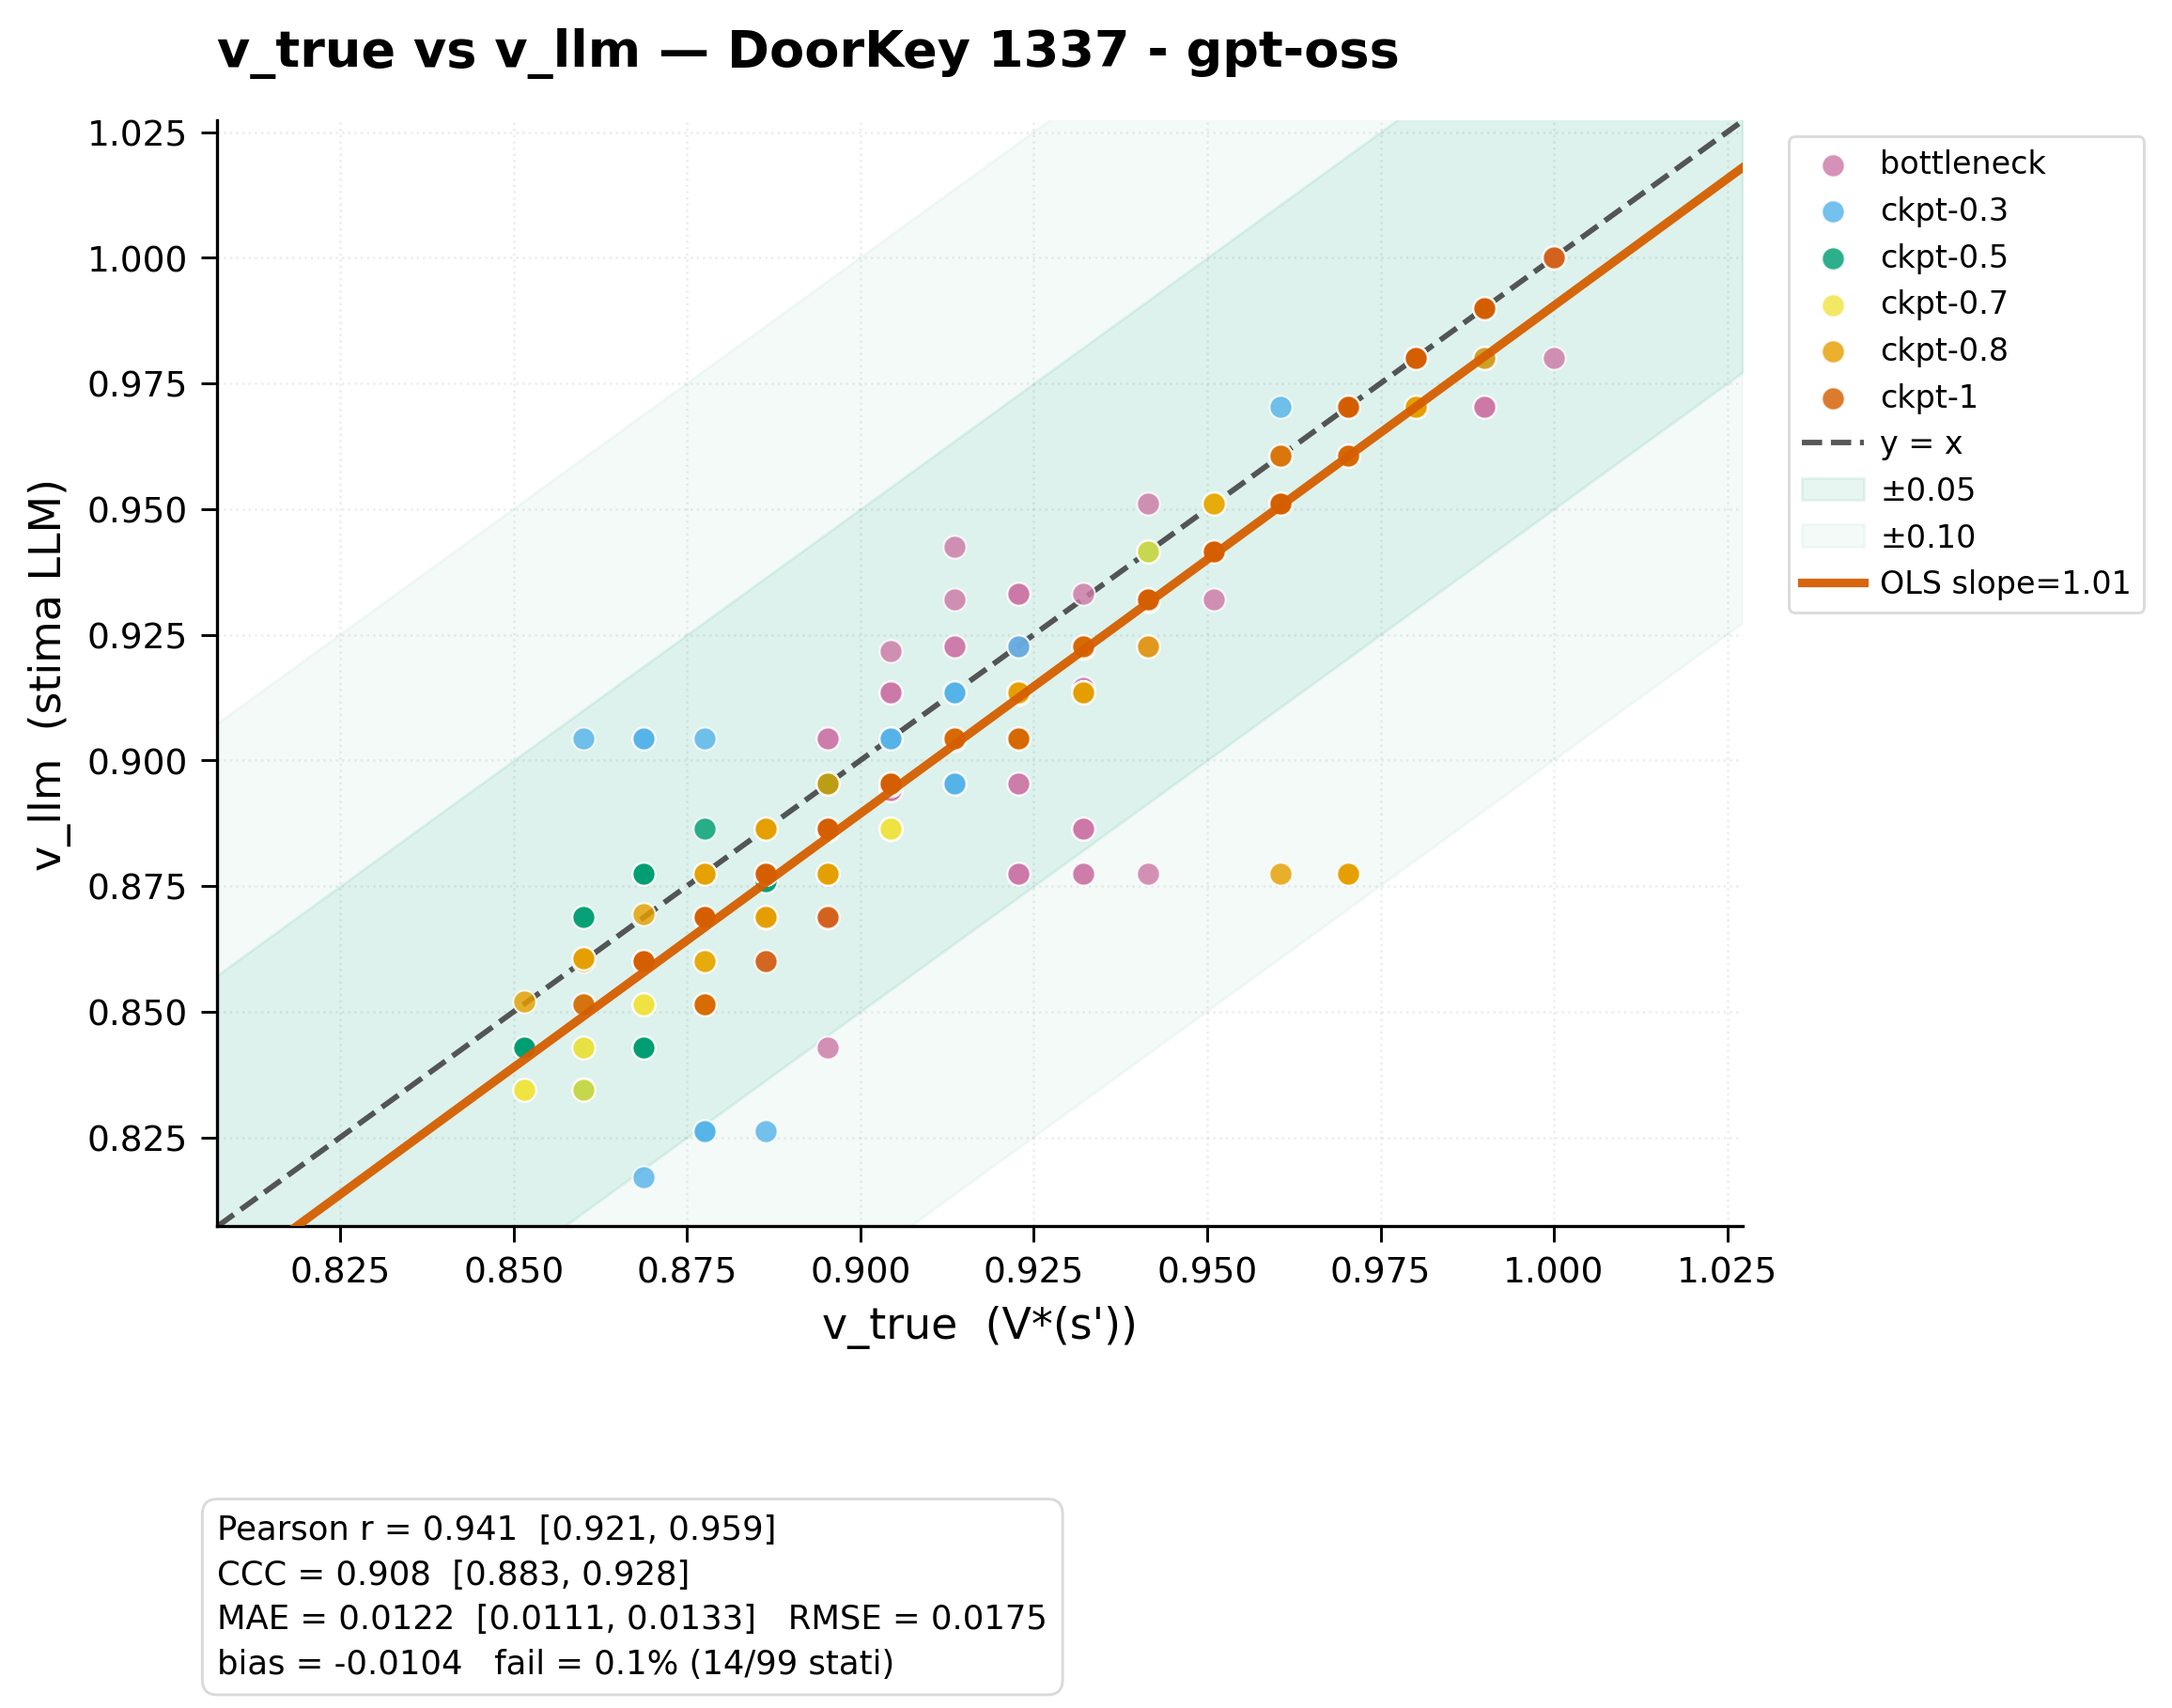
\includegraphics[width=\textwidth]{../src/output/evaluate/grafici/llm_results_doorkey_states_8x8_seed1337_gpt-oss_120b_scatter.png}
\caption{Seed 1337: $v_{true}$ contro $v_{llm}$. Punti addensati sulla diagonale, quasi tutti nella fascia $\pm 0.05$.}
\label{fig:scatter1337}
\end{figure}

\begin{figure}[htbp]
\centering
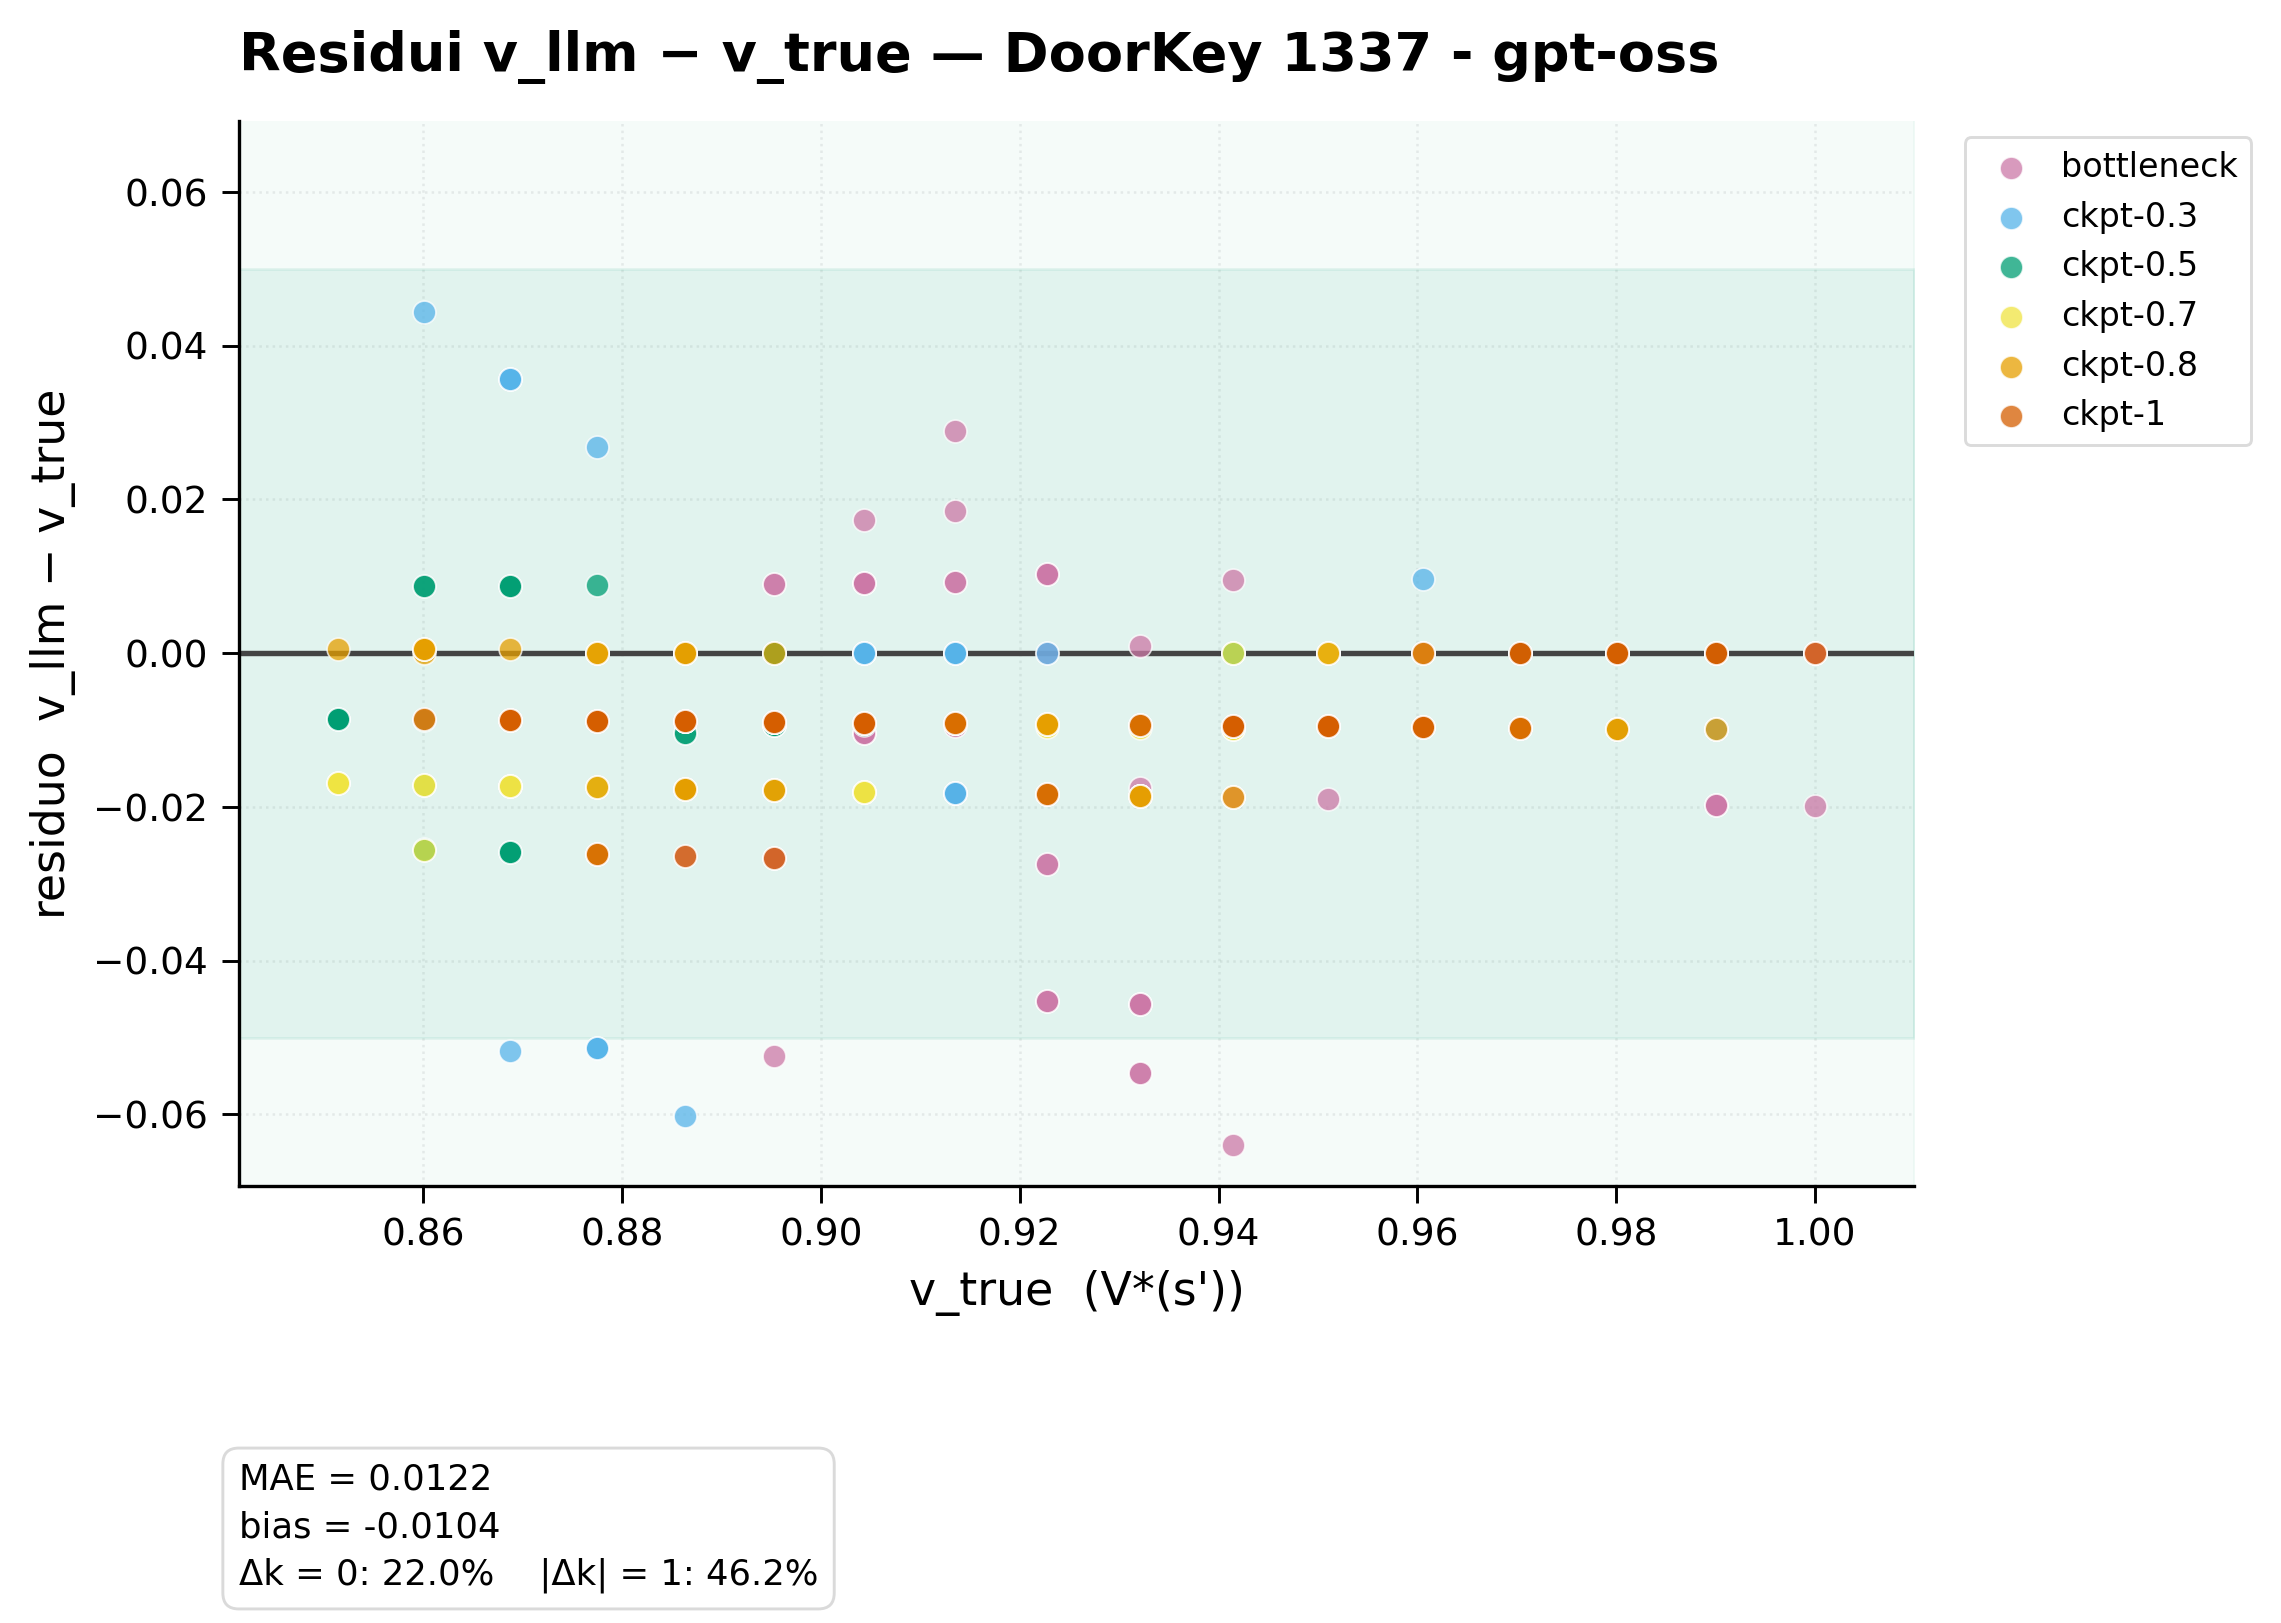
\includegraphics[width=\textwidth]{../src/output/evaluate/grafici/llm_results_doorkey_states_8x8_seed1337_gpt-oss_120b_residuals.png}
\caption{Seed 1337: residui in funzione di $v_{true}$, con bias leggermente negativo.}
\label{fig:resid1337}
\end{figure}

\begin{figure}[htbp]
\centering
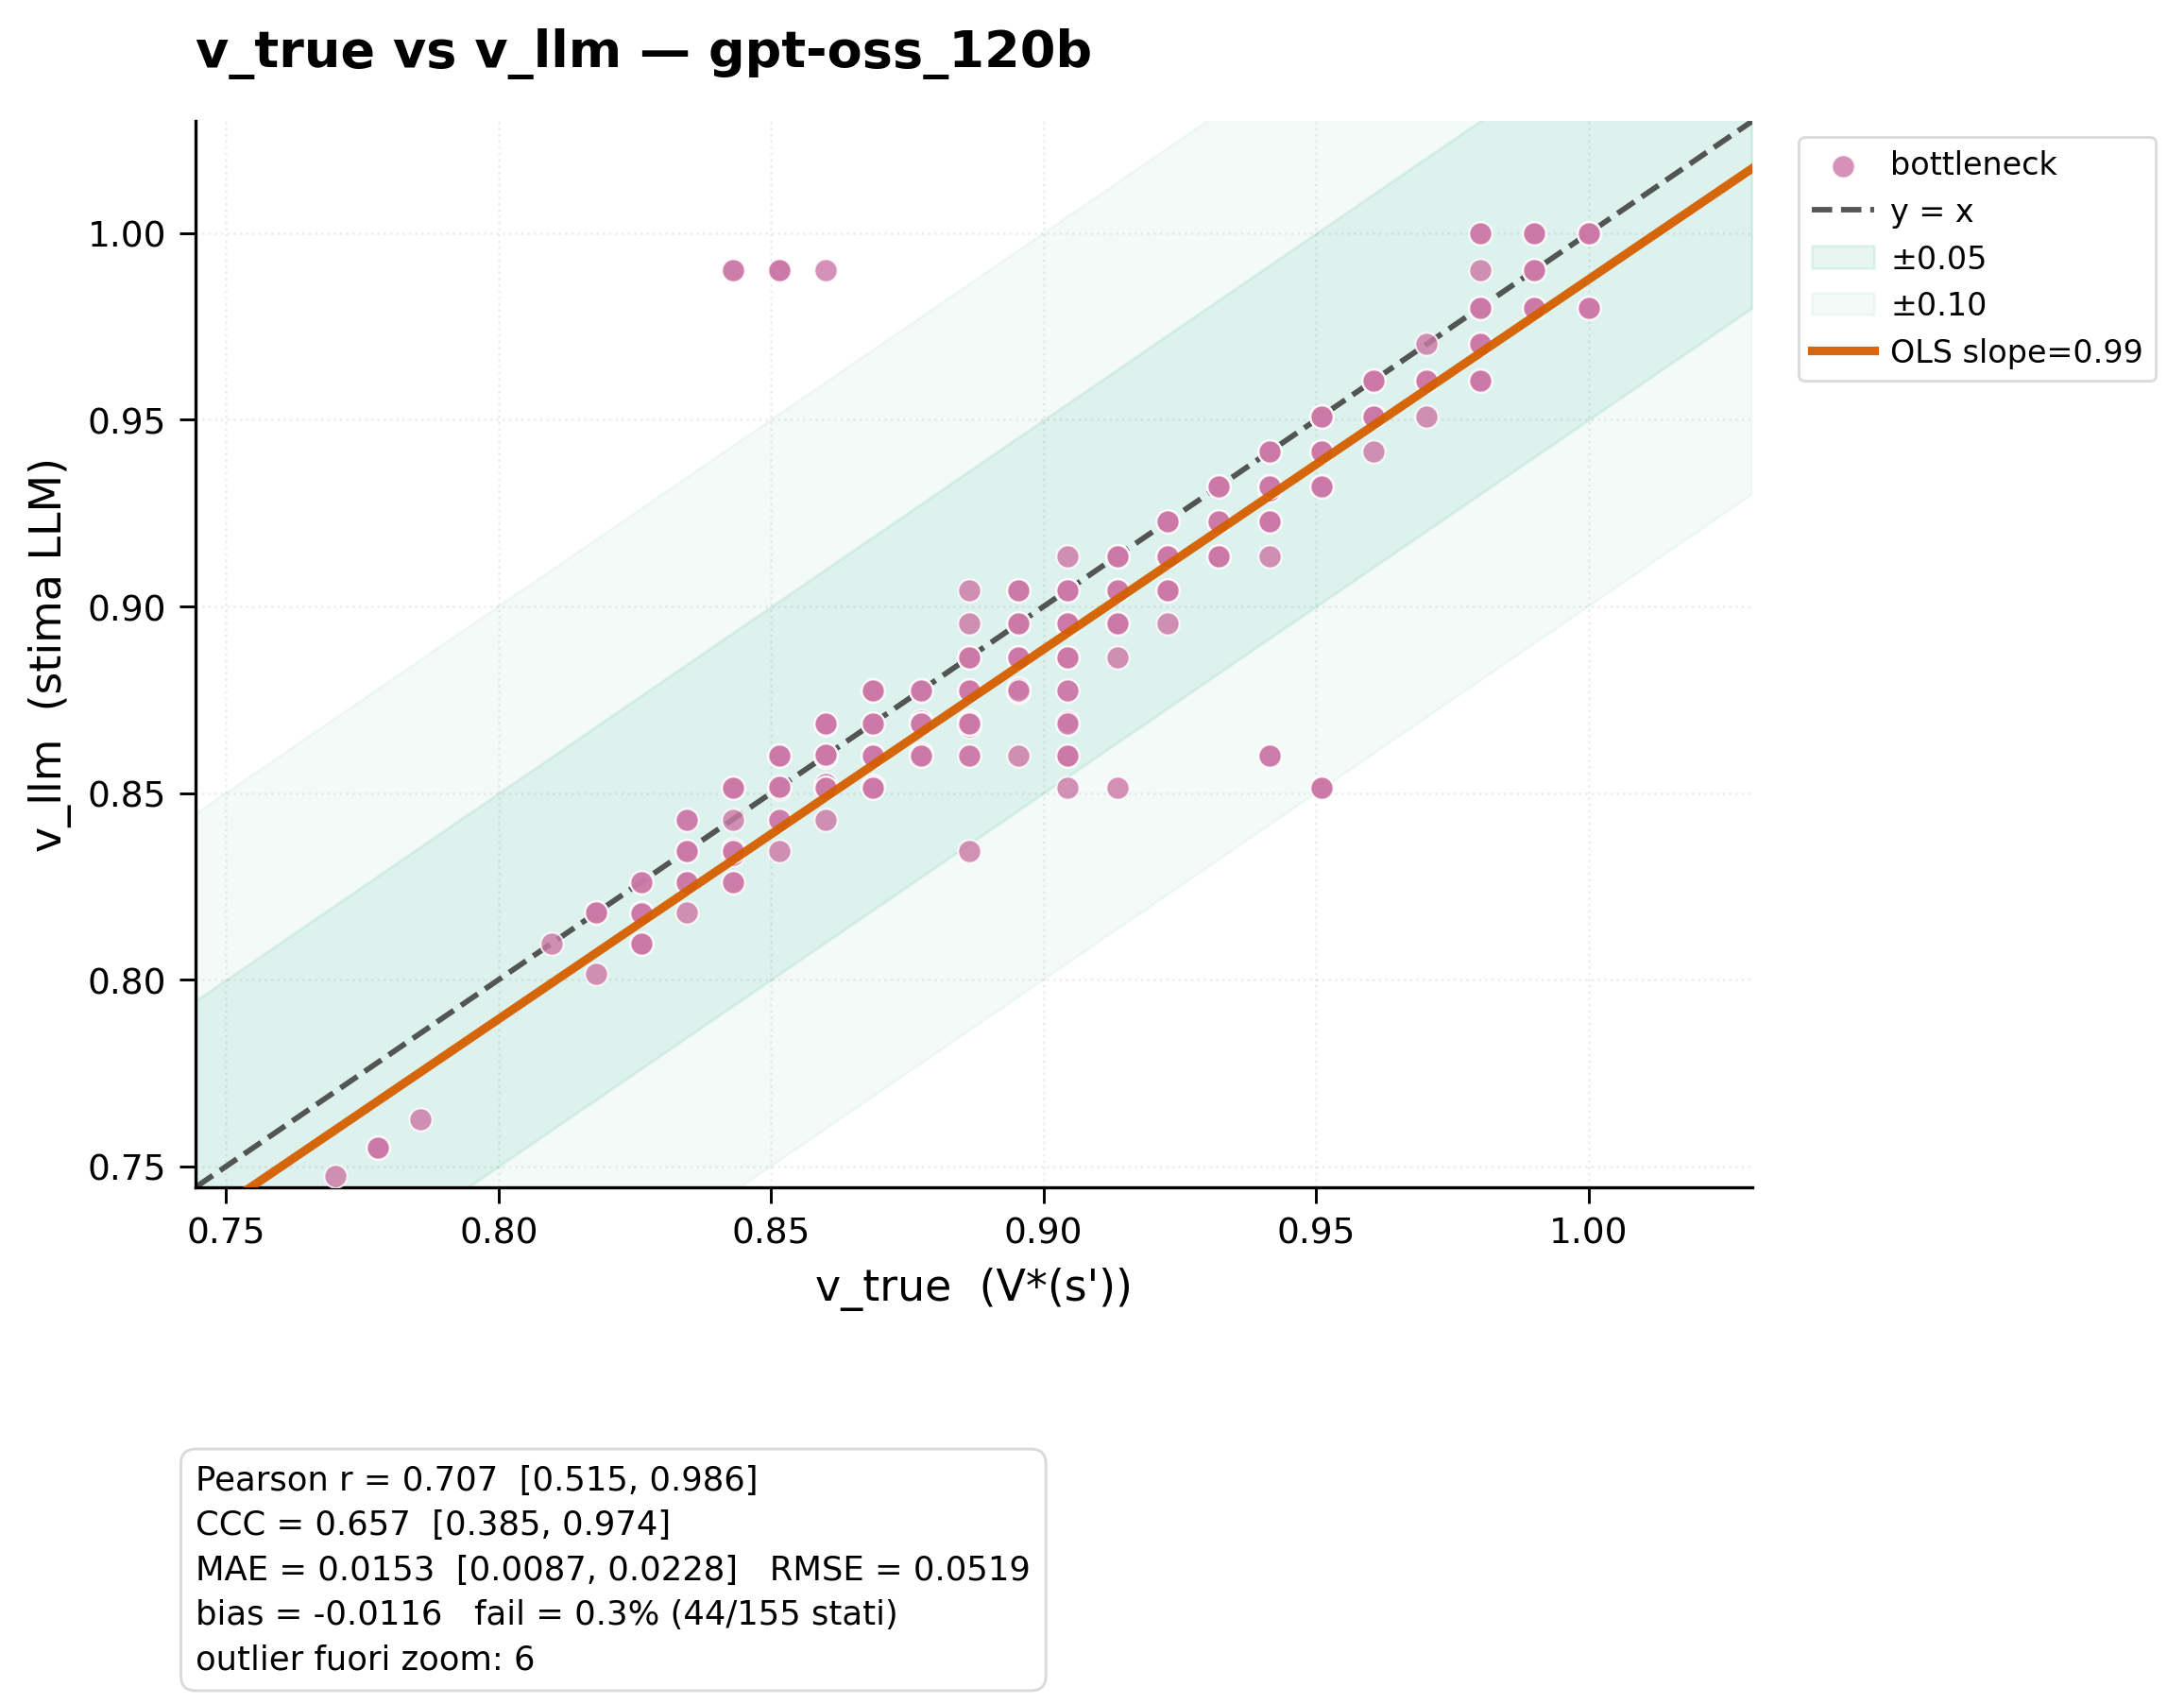
\includegraphics[width=\textwidth]{../src/output/evaluate/grafici/llm_results_doorkey_states_8x8_seeds13507-19920-32455-54937-69693_gpt-oss_120b_scatter.png}
\caption{Cinque seed, solo bottleneck: stessa diagonale, dispersione superiore.}
\label{fig:scatter5seed}
\end{figure}

\begin{figure}[htbp]
\centering
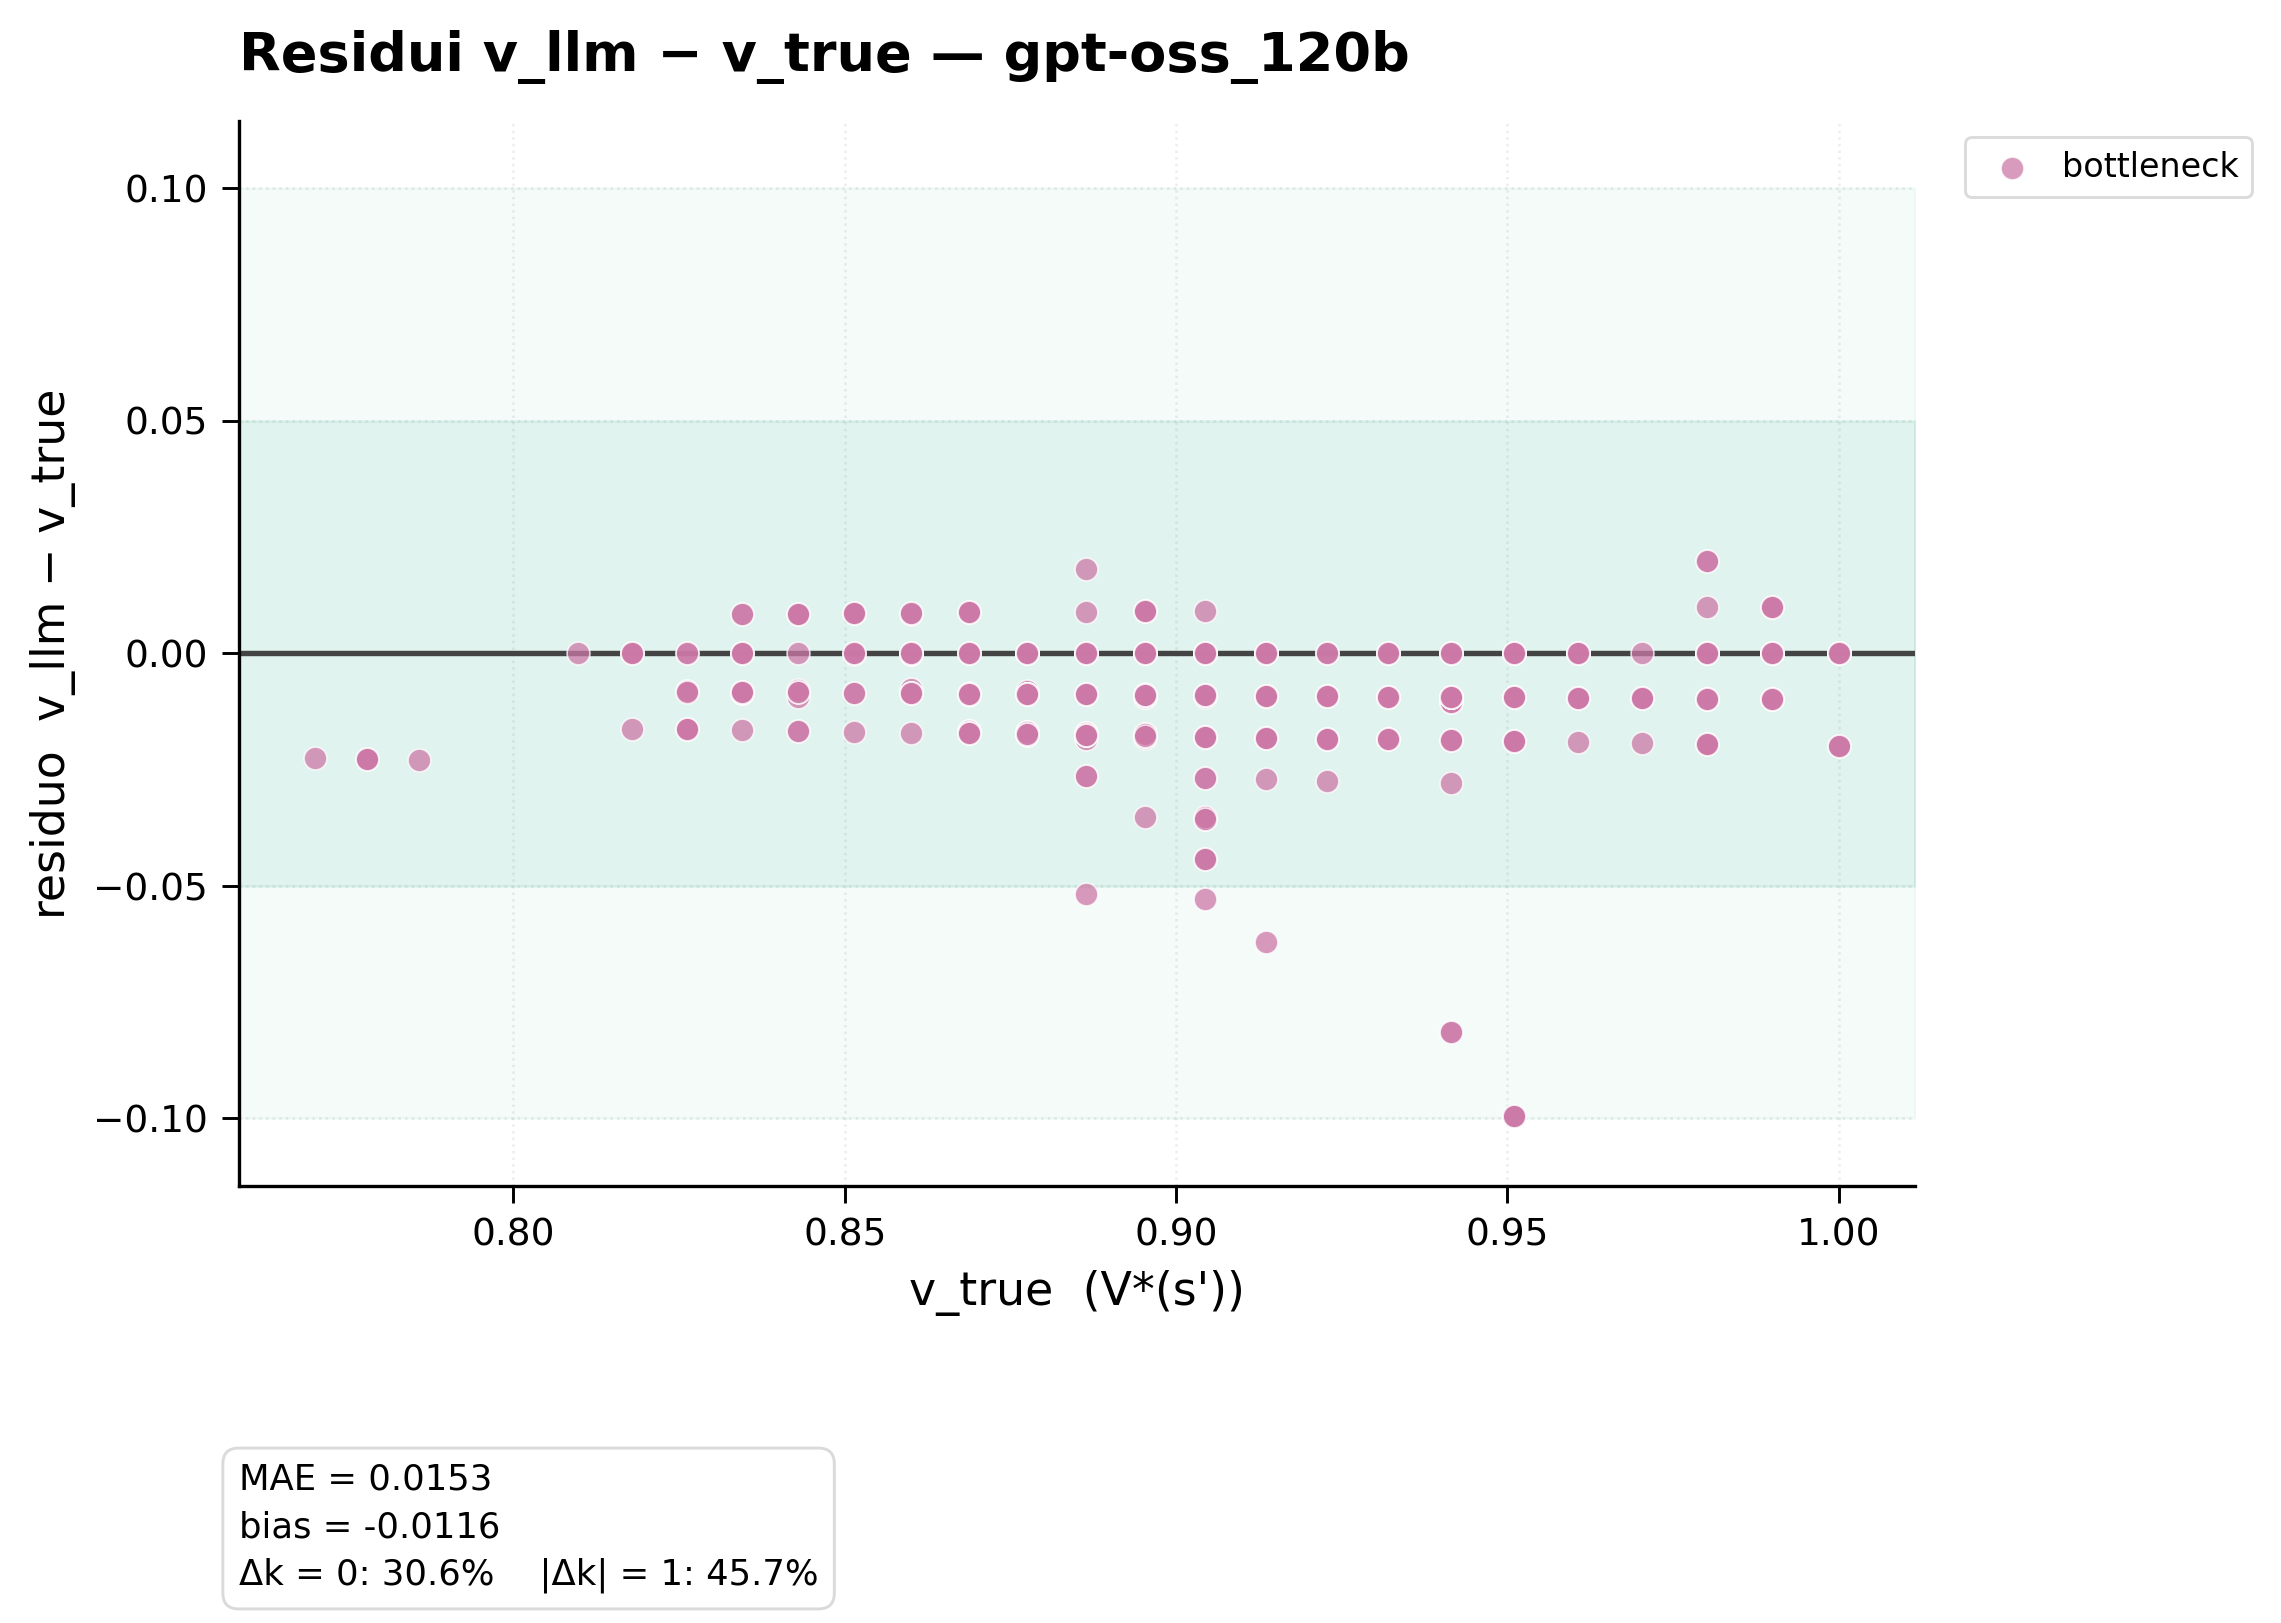
\includegraphics[width=\textwidth]{../src/output/evaluate/grafici/llm_results_doorkey_states_8x8_seeds13507-19920-32455-54937-69693_gpt-oss_120b_residuals.png}
\caption{Cinque seed, solo bottleneck: residui in funzione di $v_{true}$.}
\label{fig:resid5seed}
\end{figure}

Il bias negativo ($\approx -0.01$) indica una sottostima sistematica di circa un passo di sconto. La distribuzione delle stime \`e visibile nelle Figure~\ref{fig:scatter1337} e \ref{fig:scatter5seed}.

\section{L'azione indotta \`e quella giusta?}\label{sec:azioni}
La verifica considera il massimo con tolleranza per i pari merito (nel codice \path{tie-aware}: \`e corretta una qualsiasi delle azioni a pari valore secondo quantizzazione su $\gamma^k$):
\begin{itemize}
\item seed 1337: Top-1 al 94.1\%, in senso stretto 84.7\%, Top-2 al 98.8\%. Il livello casuale su 6 azioni \`e 16.7\%.
\item rimpianto medio 0.0011: gli errori comportano una perdita attesa contenuta.
\item bottleneck 82.8\%, tutti i checkpoint al 100\%.
\end{itemize}
$\Delta k$ pari a zero nel 22.0\% dei casi, a $\pm 1$ nel 46.2\%: i valori assoluti risultano accurati, la distanza in passi in misura minore. Il quadro per gruppo \`e nelle Figure~\ref{fig:acc1337} e \ref{fig:acc5seed}.

Cinque seed: Top-1 al 91.9\%, in senso stretto 82.0\%, Top-2 al 96.4\%, rimpianto 0.0020.

\begin{figure}[h]
\centering
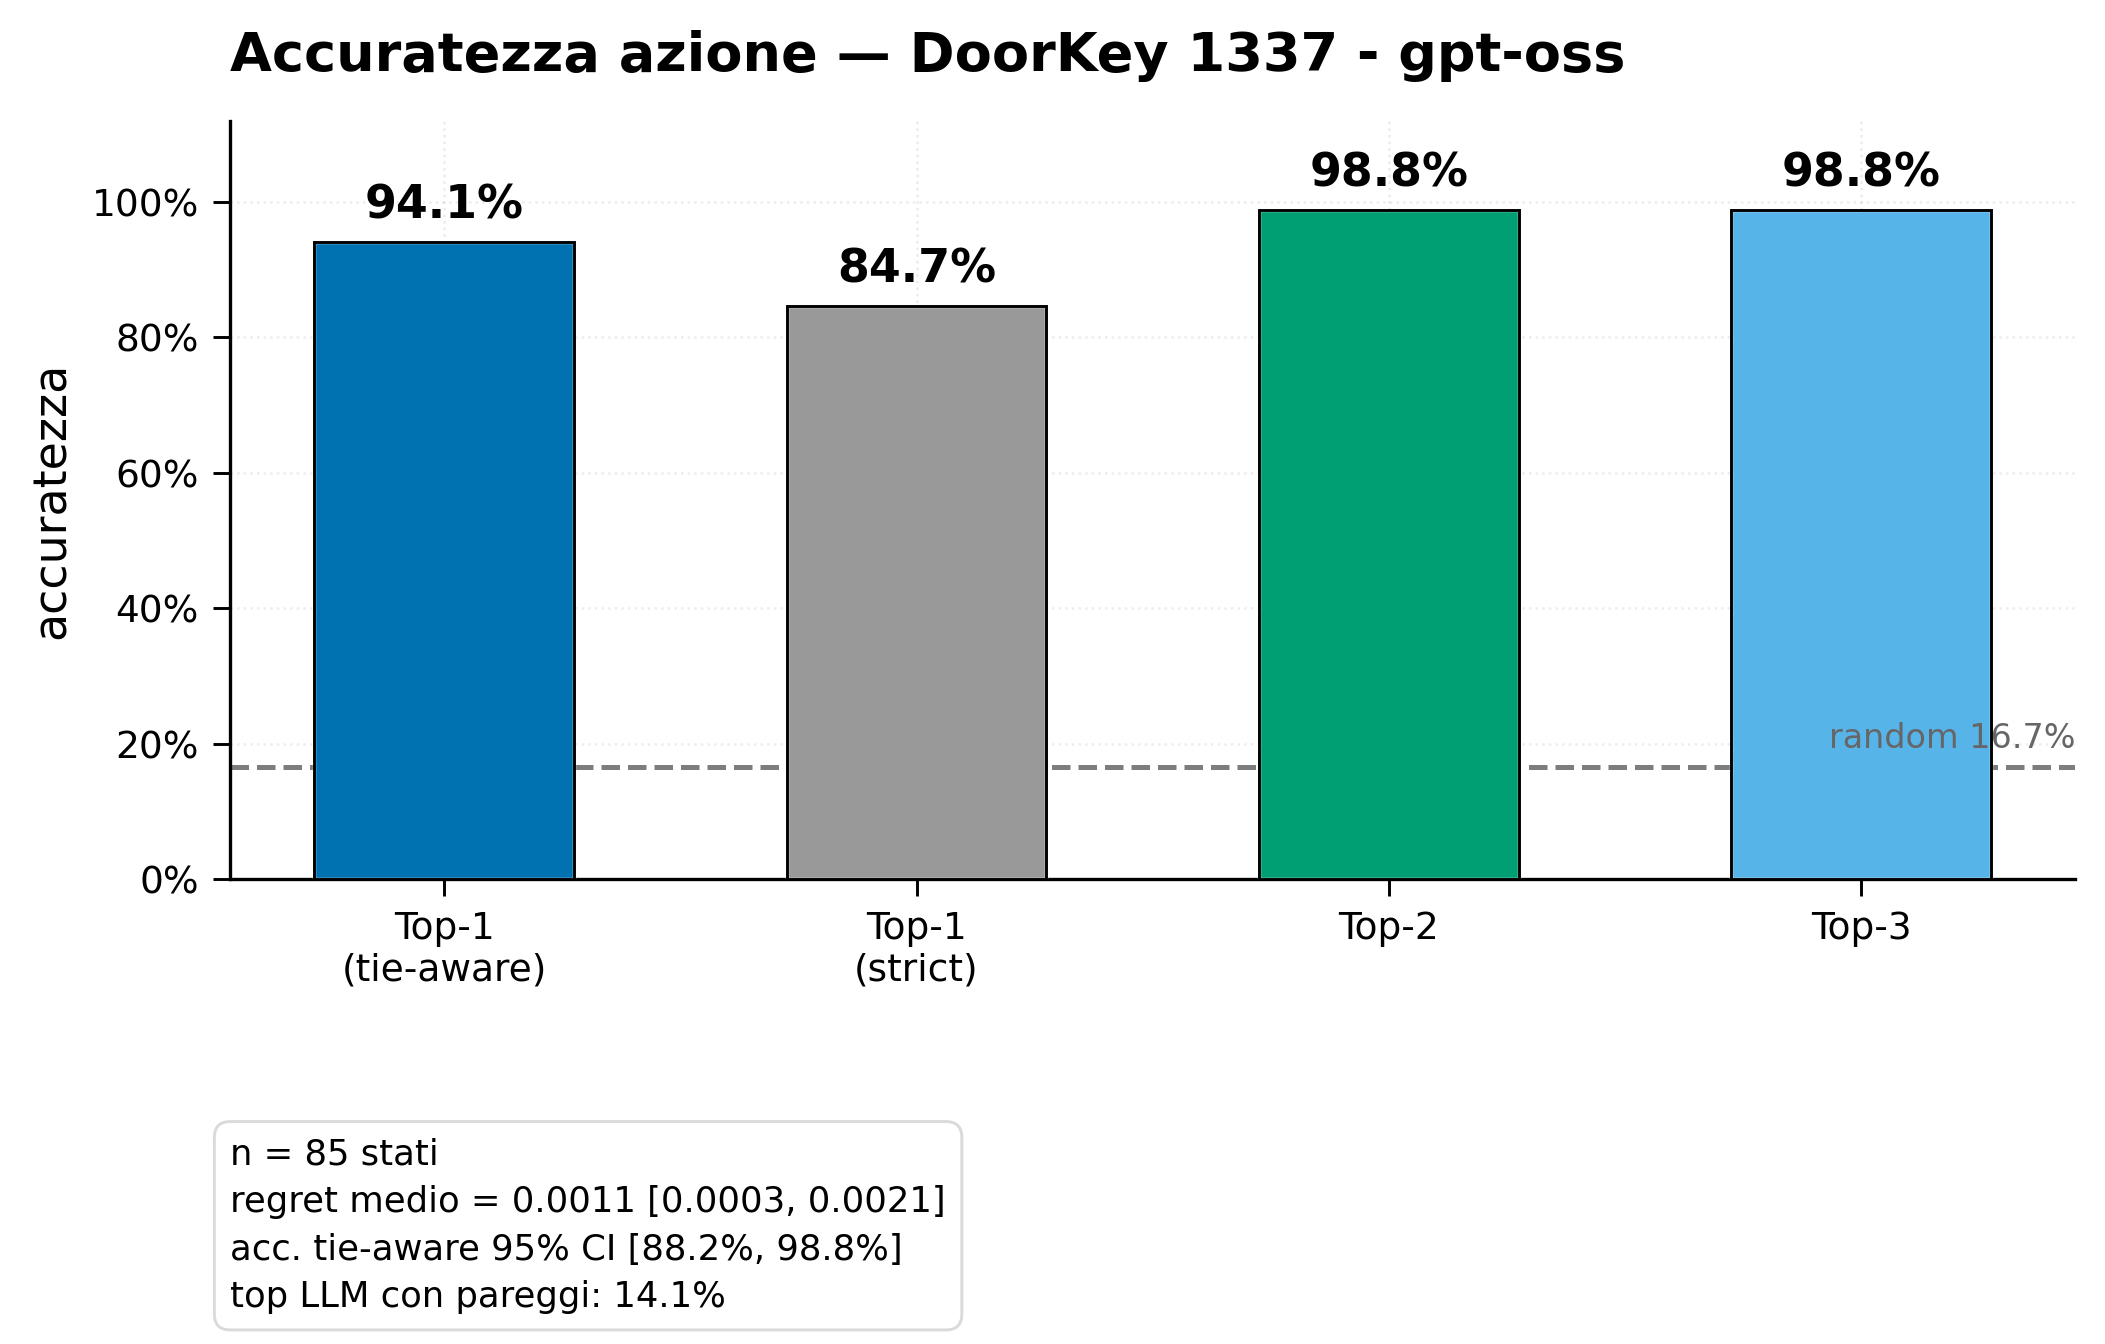
\includegraphics[width=0.48\textwidth]{../src/output/evaluate/grafici/llm_results_doorkey_states_8x8_seed1337_gpt-oss_120b_accuracy.png}
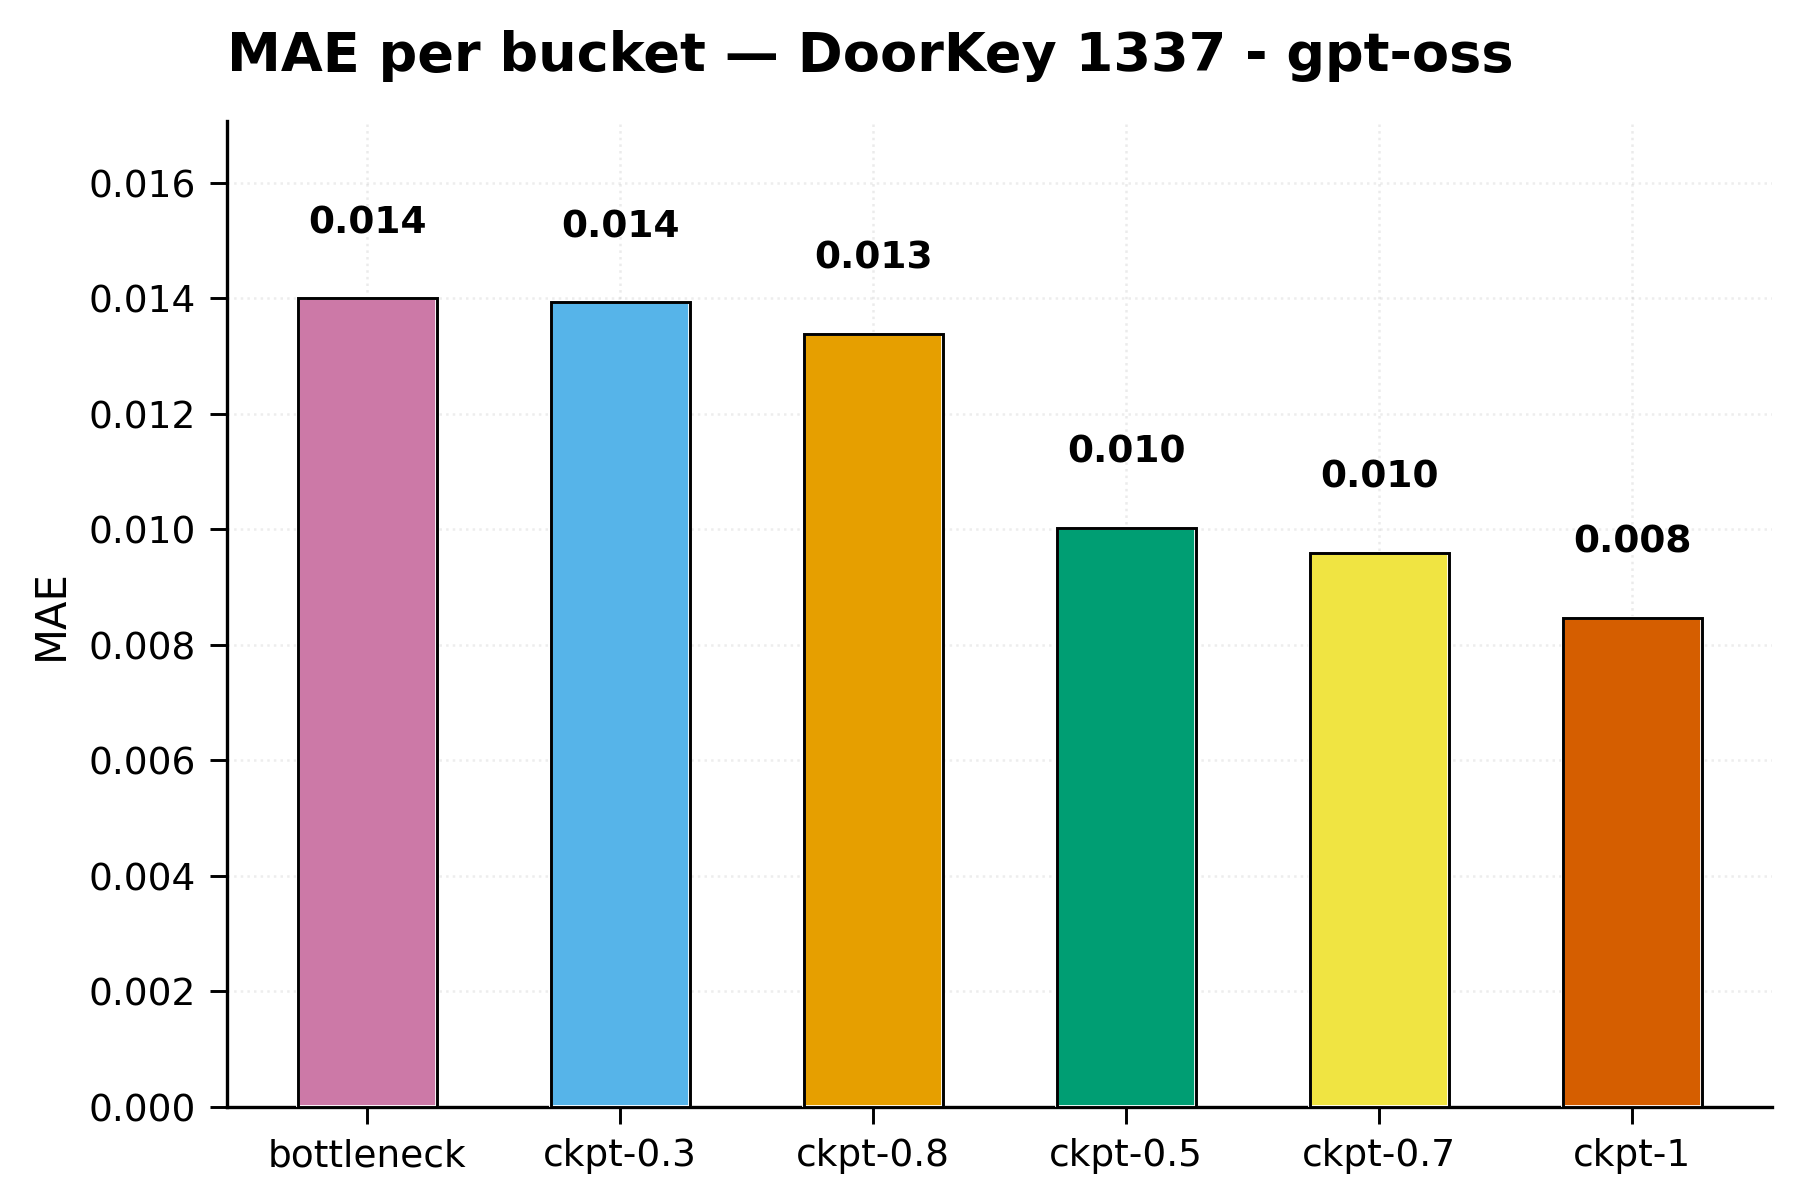
\includegraphics[width=0.48\textwidth]{../src/output/evaluate/grafici/llm_results_doorkey_states_8x8_seed1337_gpt-oss_120b_mae_bucket.png}
\caption{Seed 1337: accuratezza e errore per gruppo. I bottleneck presentano l'errore maggiore.}
\label{fig:acc1337}
\end{figure}

\begin{figure}[h]
\centering
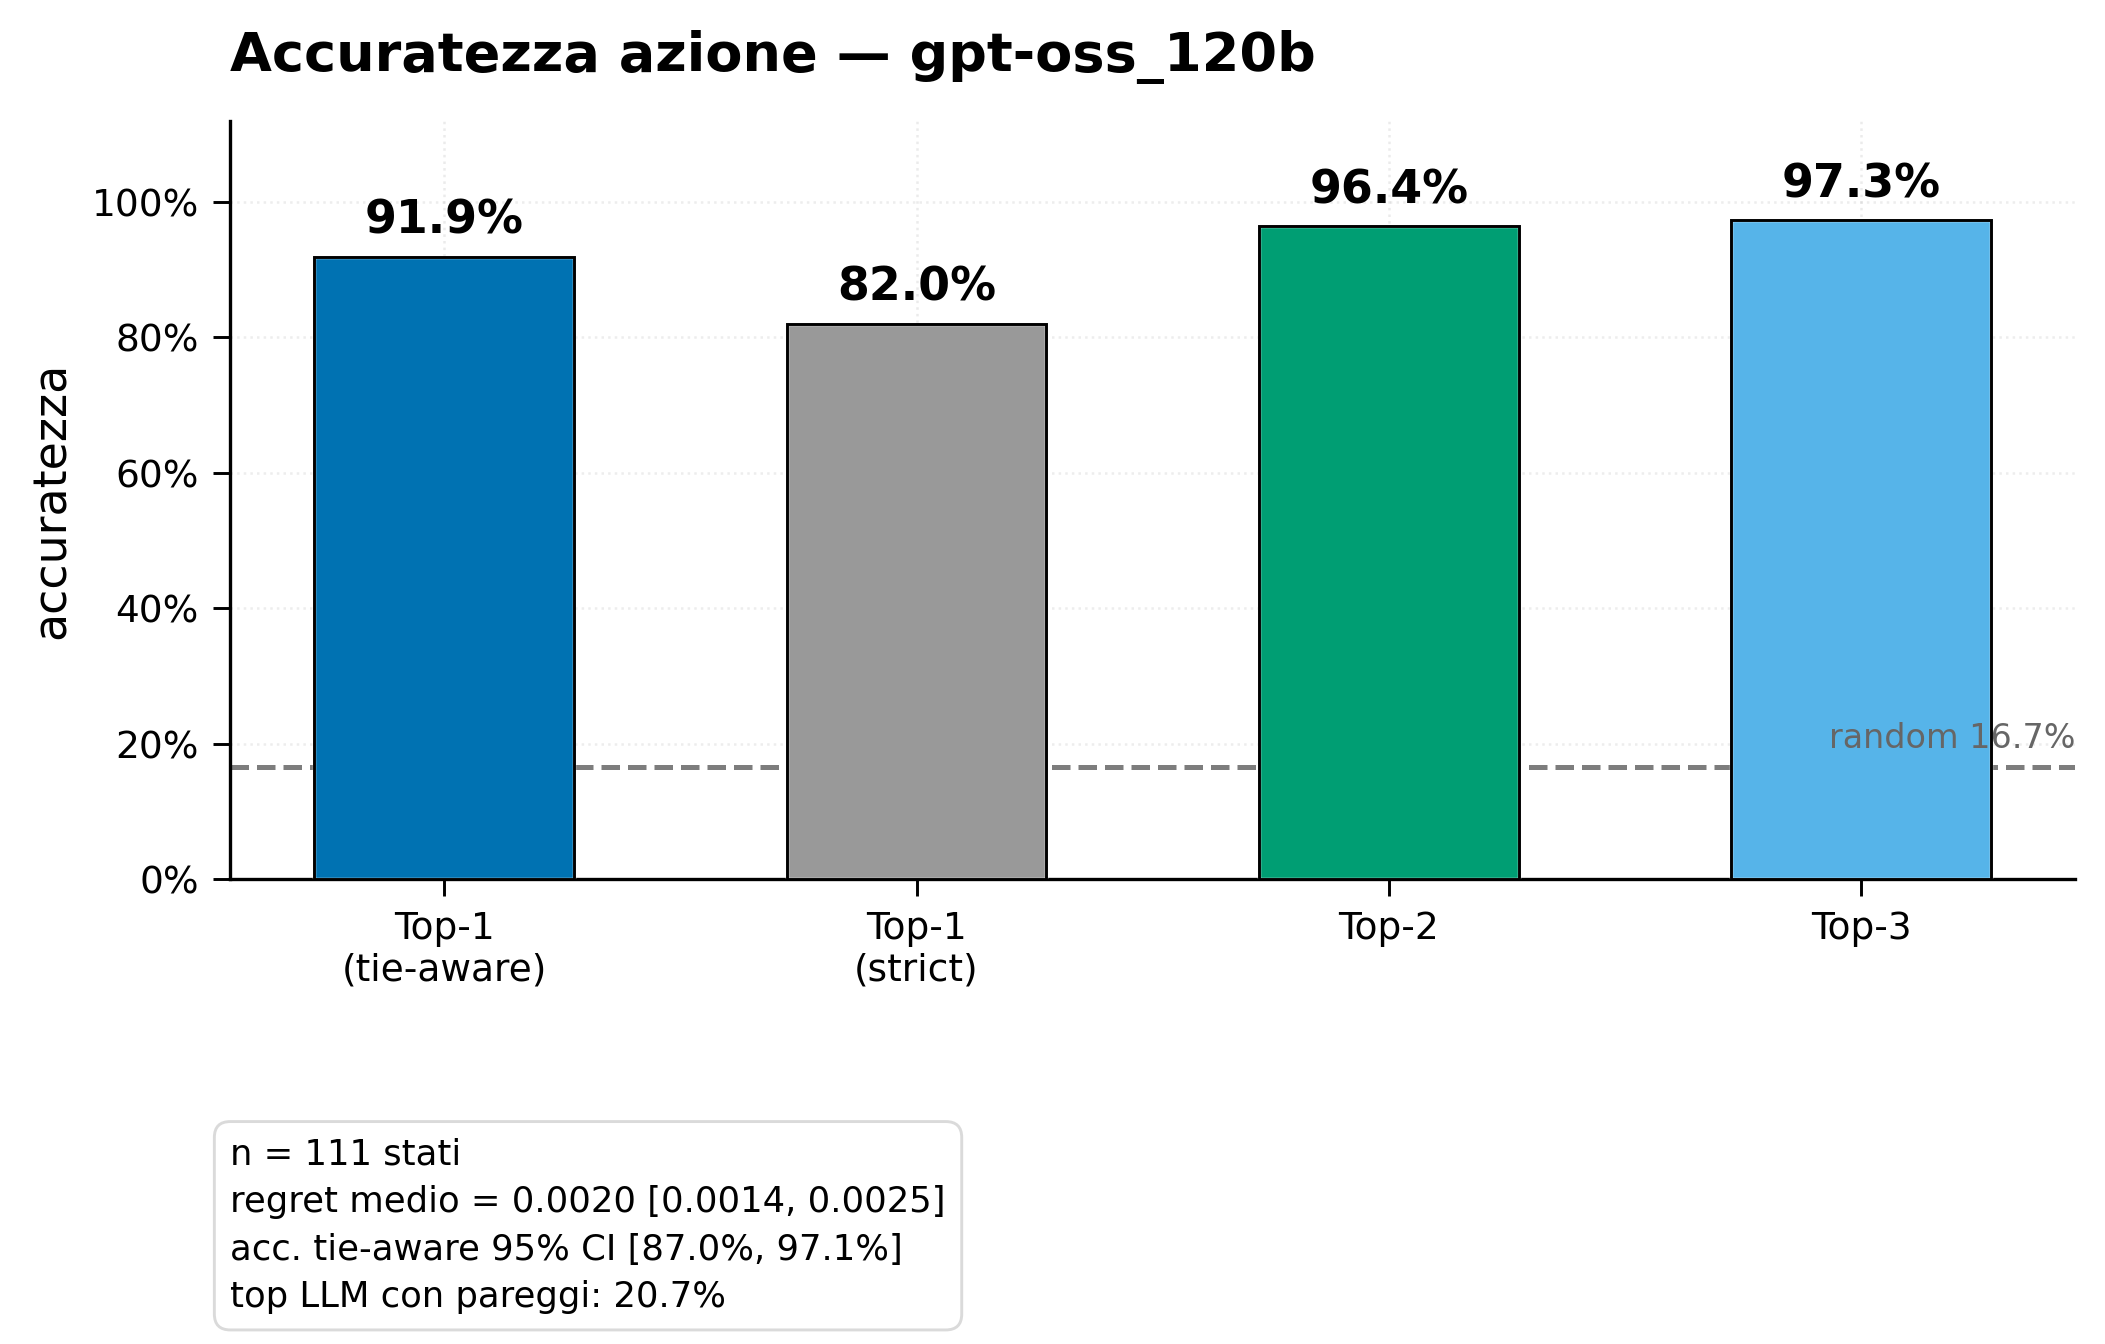
\includegraphics[width=0.48\textwidth]{../src/output/evaluate/grafici/llm_results_doorkey_states_8x8_seeds13507-19920-32455-54937-69693_gpt-oss_120b_accuracy.png}
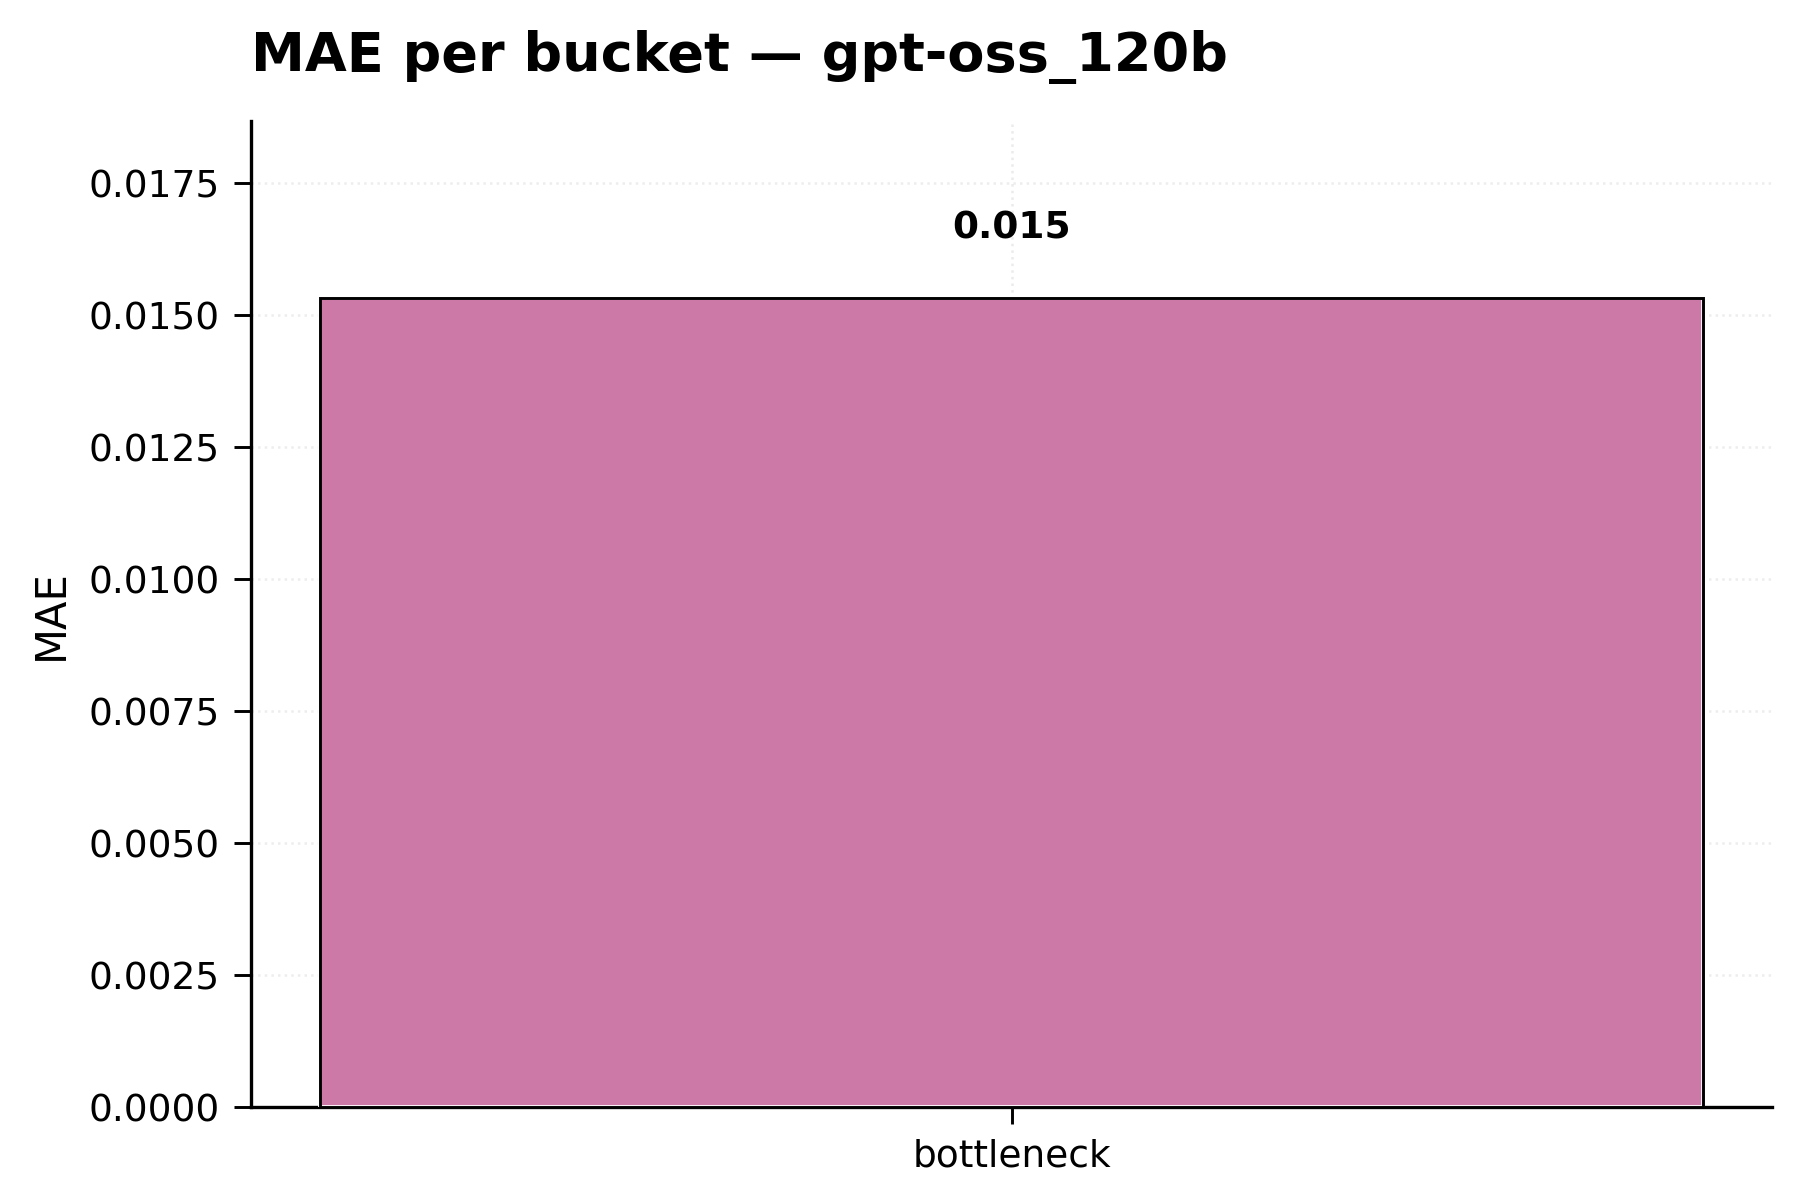
\includegraphics[width=0.48\textwidth]{../src/output/evaluate/grafici/llm_results_doorkey_states_8x8_seeds13507-19920-32455-54937-69693_gpt-oss_120b_mae_bucket.png}
\caption{Cinque seed, solo bottleneck: Top-1 91.9\%, Top-2 96.4\%.}
\label{fig:acc5seed}
\end{figure}

\section{Effetto dell'inizializzazione}\label{sec:init}
L'agente \`e implementato in \path{src/agent/doorkey_qtable_llminit.py} e opera in coordinate relative al bersaglio di fase \path{(dx, dy, dir, stage)}, in modo che righe corrispondenti su seed differenti condividano la tabella. Le coppie coperte partono dalla media delle stime, le rimanenti da zero. L'apprendimento successivo \`e Q-learning ordinario, con i bottleneck di valore maggiore per primi (\path{bottleneck_first_top_v}).

La qualit\`a della politica appresa viene misurata contro la politica ottima da value iteration con due metriche (\path{optimal_policy_metrics} in \path{src/agent/doorkey_qtable_llminit.py}). L'accordo indica la frazione degli stati visitati e mappati in cui l'azione greedy appresa coincide con un'azione ottima, a meno di tolleranza $10^{-6}$ per i pari merito: vale 1 se la politica appresa sceglie sempre un'azione ottima sugli stati valutati. La perdita di valore \`e la media, sugli stessi stati, di $V^*(s)-Q^*(s,a)$ con $a$ azione appresa: quanto valore atteso si perde seguendo la politica appresa invece dell'ottima, in unit\`a di ricompensa scontata. Con $\gamma=0.99$ un passo sprecato vale circa 0.01, quindi una perdita media di 0.0067 corrisponde a meno di un passo perso in media. Entrambe sono calcolate solo sugli stati visitati e mappati, con terminali esclusi: descrivono la qualit\`a dove l'agente \`e passato, non sull'intero grafo.

Configurazione principale, seed 1337, 2000 episodi, $\alpha=0.07$, $\gamma=0.9$, decadimento di $\epsilon$ 0.99, \path{max_init=20}. Sono 20 coppie dai bottleneck, il 4\% dei 480 nodi:
\begin{itemize}
\item con inizializzazione: valutazione 1.00, 17 passi medi, accordo con l'ottima 0.585, perdita 0.0067;
\item controllo senza inizializzazione, stessi iperparametri: valutazione 0.00, 450 passi, accordo 0.481;
\item controllo senza inizializzazione con iperparametri standard ($\alpha=0.25$, $\gamma=0.99$): valutazione 1.00, 16 passi, accordo 0.556.
\end{itemize}
A pari iperparametri la configurazione senza inizializzazione non risolve il compito: la differenza osservata \`e attribuibile all'inizializzazione (Figure~\ref{fig:samehp} e \ref{fig:vstd}). Con gli iperparametri standard anche il controllo risolve, con un passo in meno (16 contro 17).

\begin{figure}[htbp]
\centering
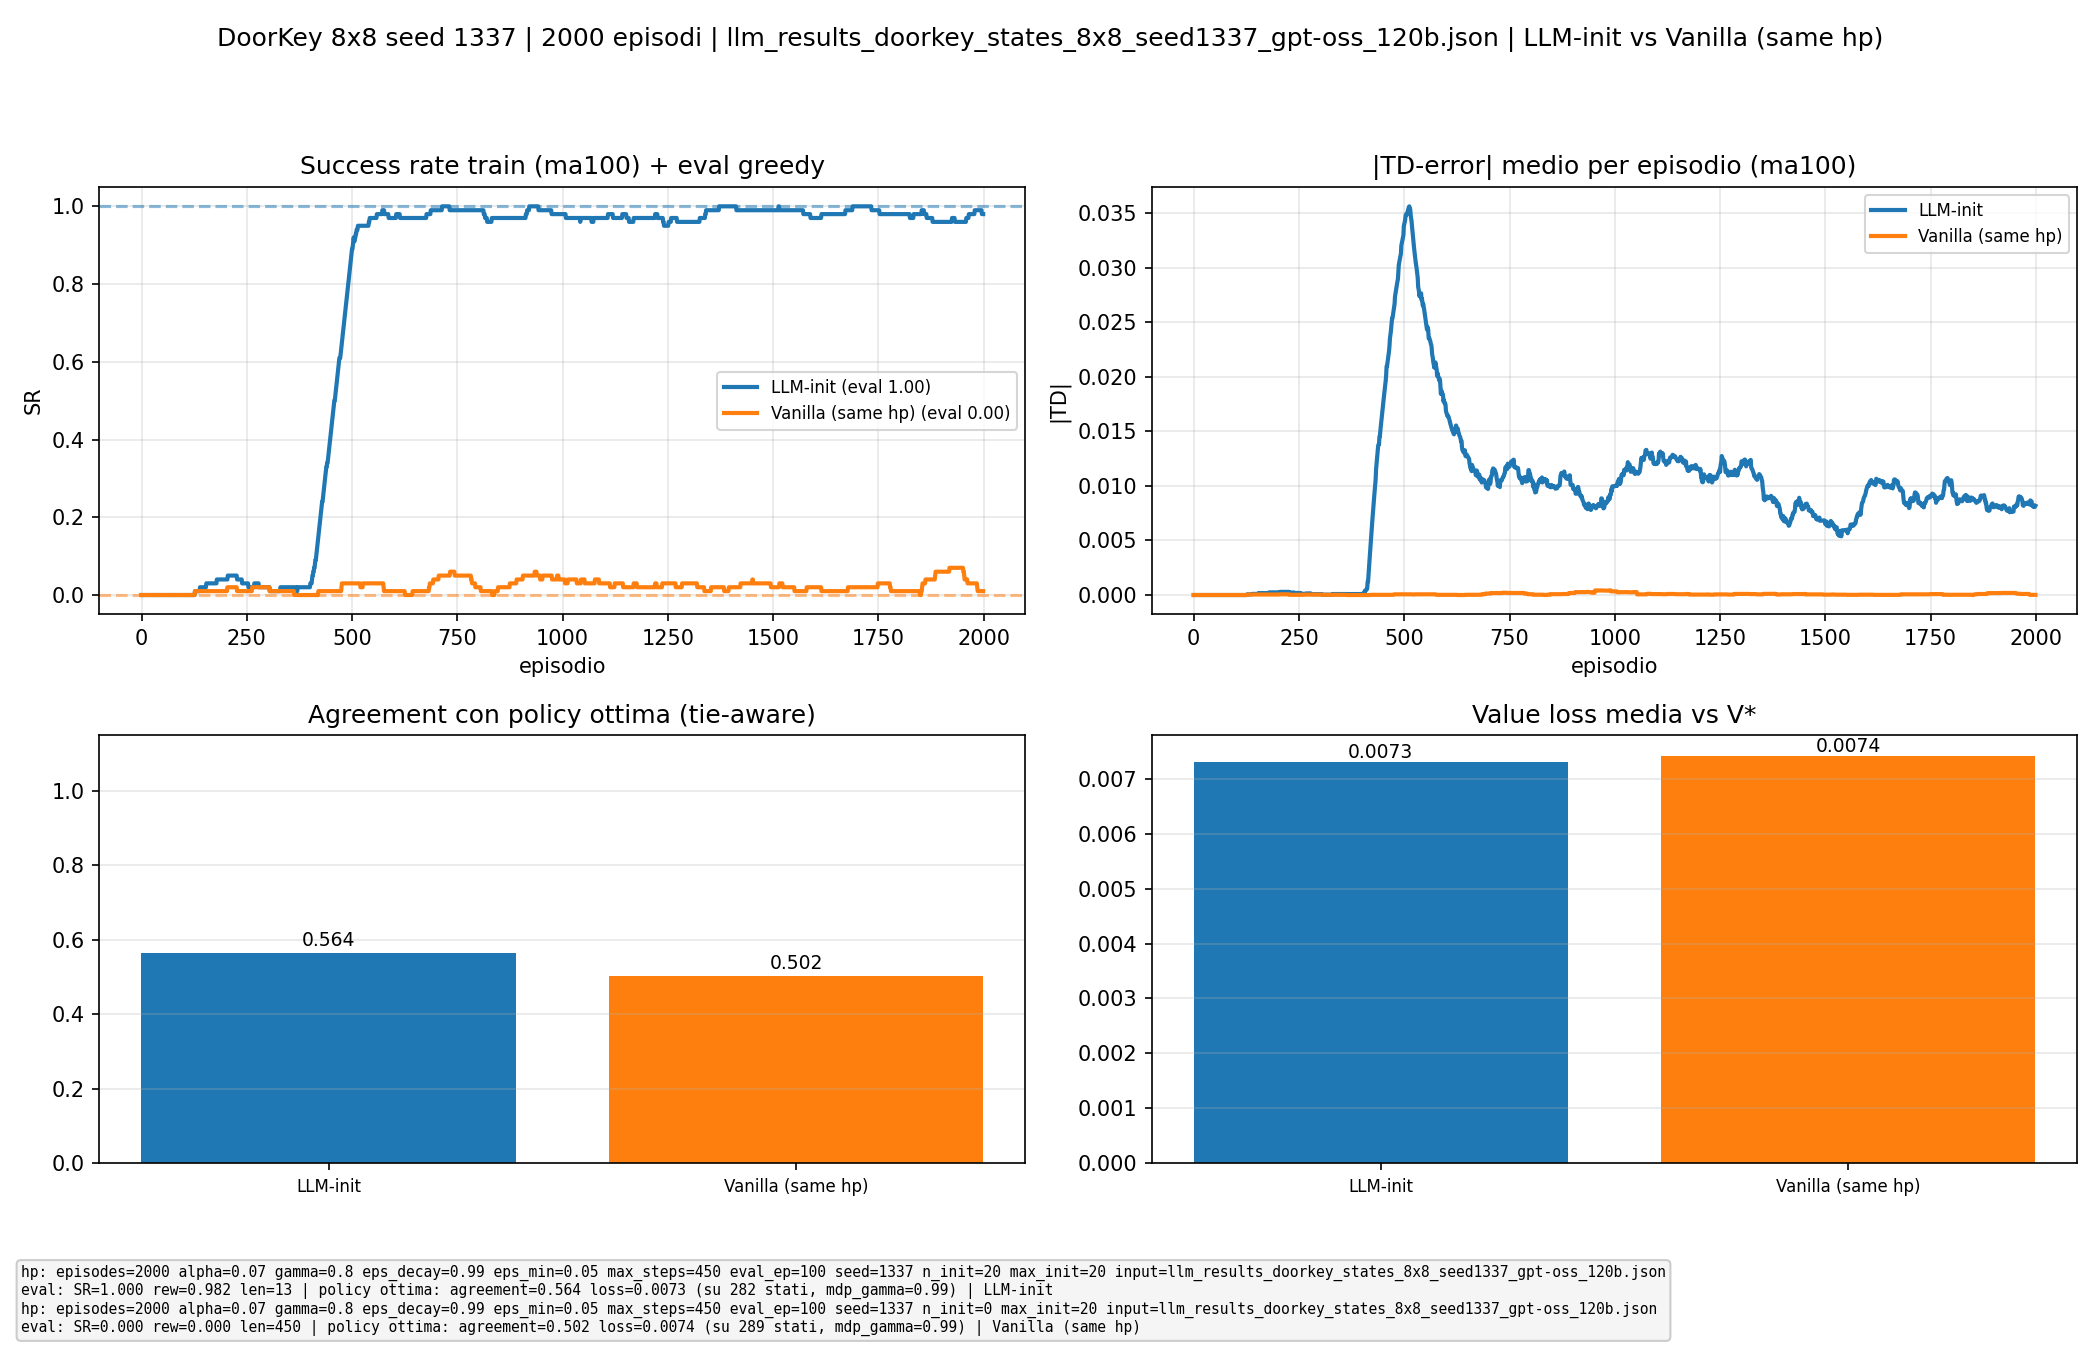
\includegraphics[width=\textwidth]{../src/output/agents/qtable_llminit_seed_1337_gpt-oss_120b_vs_samehp.png}
\caption{Seed 1337, confronto a pari iperparametri tra inizializzazione da modello e controllo: il controllo resta a tasso nullo.}
\label{fig:samehp}
\end{figure}

\begin{figure}[htbp]
\centering
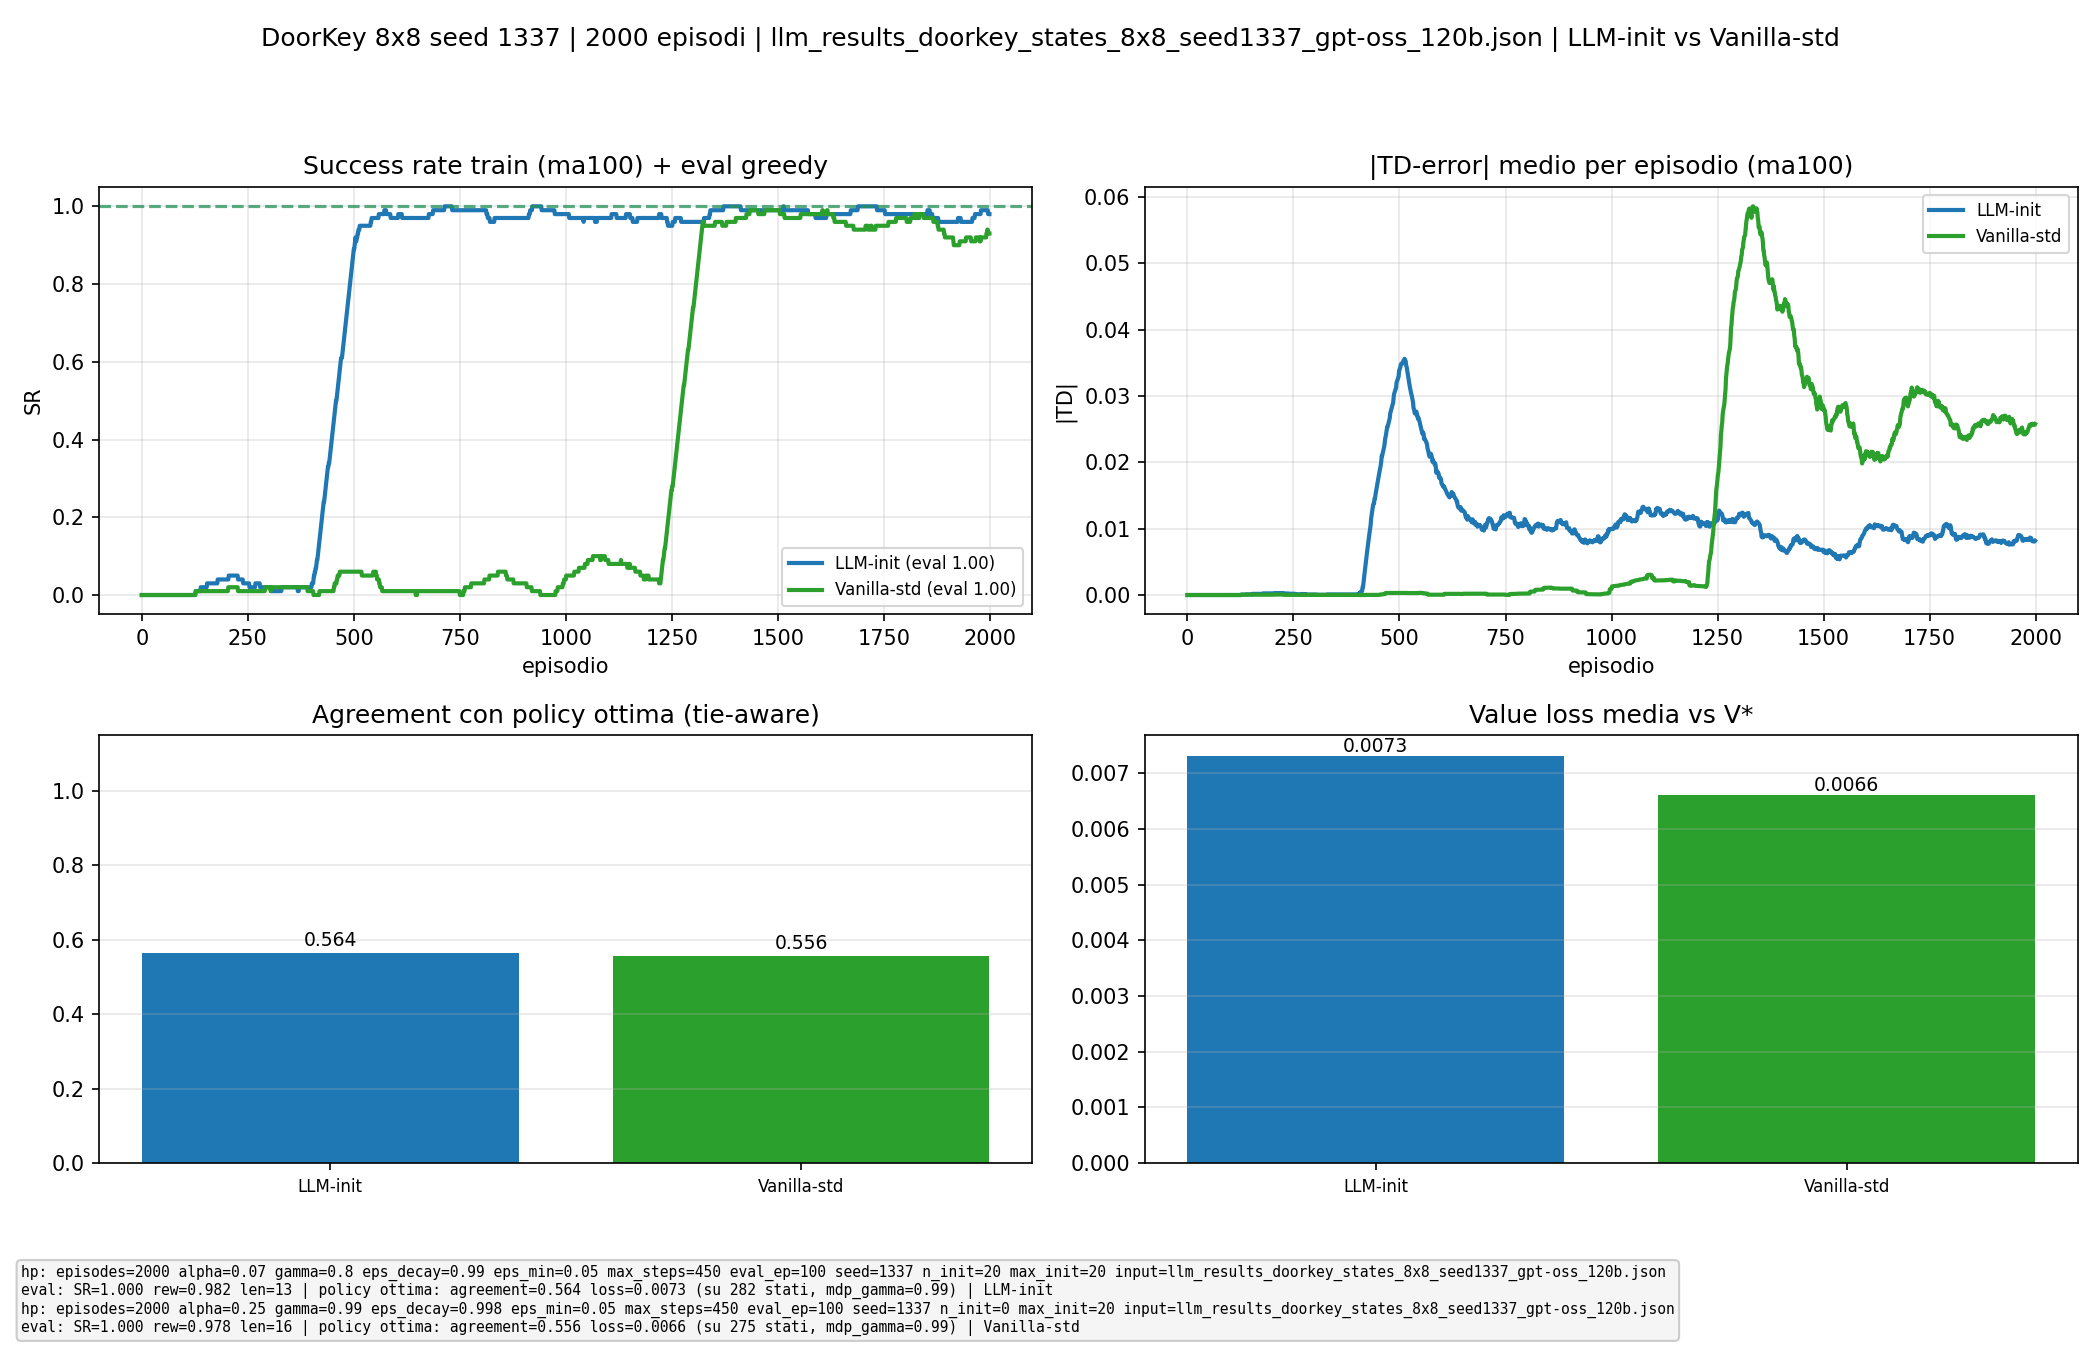
\includegraphics[width=\textwidth]{../src/output/agents/qtable_llminit_seed_1337_gpt-oss_120b_vs_std.png}
\caption{Seed 1337, confronto con il controllo a iperparametri standard: entrambi risolvono, con 17 passi medi contro 16.}
\label{fig:vstd}
\end{figure}

Secondo esperimento: addestramento sui cinque seed 13507, 19920, 32455, 54937 e 69693 in coordinate relative (4000 episodi, $\alpha=0.1$, $\gamma=0.8$, decadimento di $\epsilon$ 0.998, \path{max_init=500}, 500 coppie), con valutazione sul seed interno 13507 e sul seed nuovo 6499, file nella cartella \path{src/output/agents/}:\\
\path{qtable_llminit_multiseed_train13507-19920-32455-54937-69693_evalin13507_evalnew6499_llminit.json}. Il tasso sui seed di addestramento \`e 1.00 con 23 passi medi, sul seed nuovo 0.00 con 450; i controlli senza inizializzazione ottengono 0.00 in entrambi i casi, sia a pari iperparametri sia con iperparametri standard. Cinque seed bastano a risolvere i layout visti, ma per generalizzare ne servono molti di pi\`u (Figure~\ref{fig:multisamehp} e \ref{fig:multivstd}).

\begin{figure}[htbp]
\centering
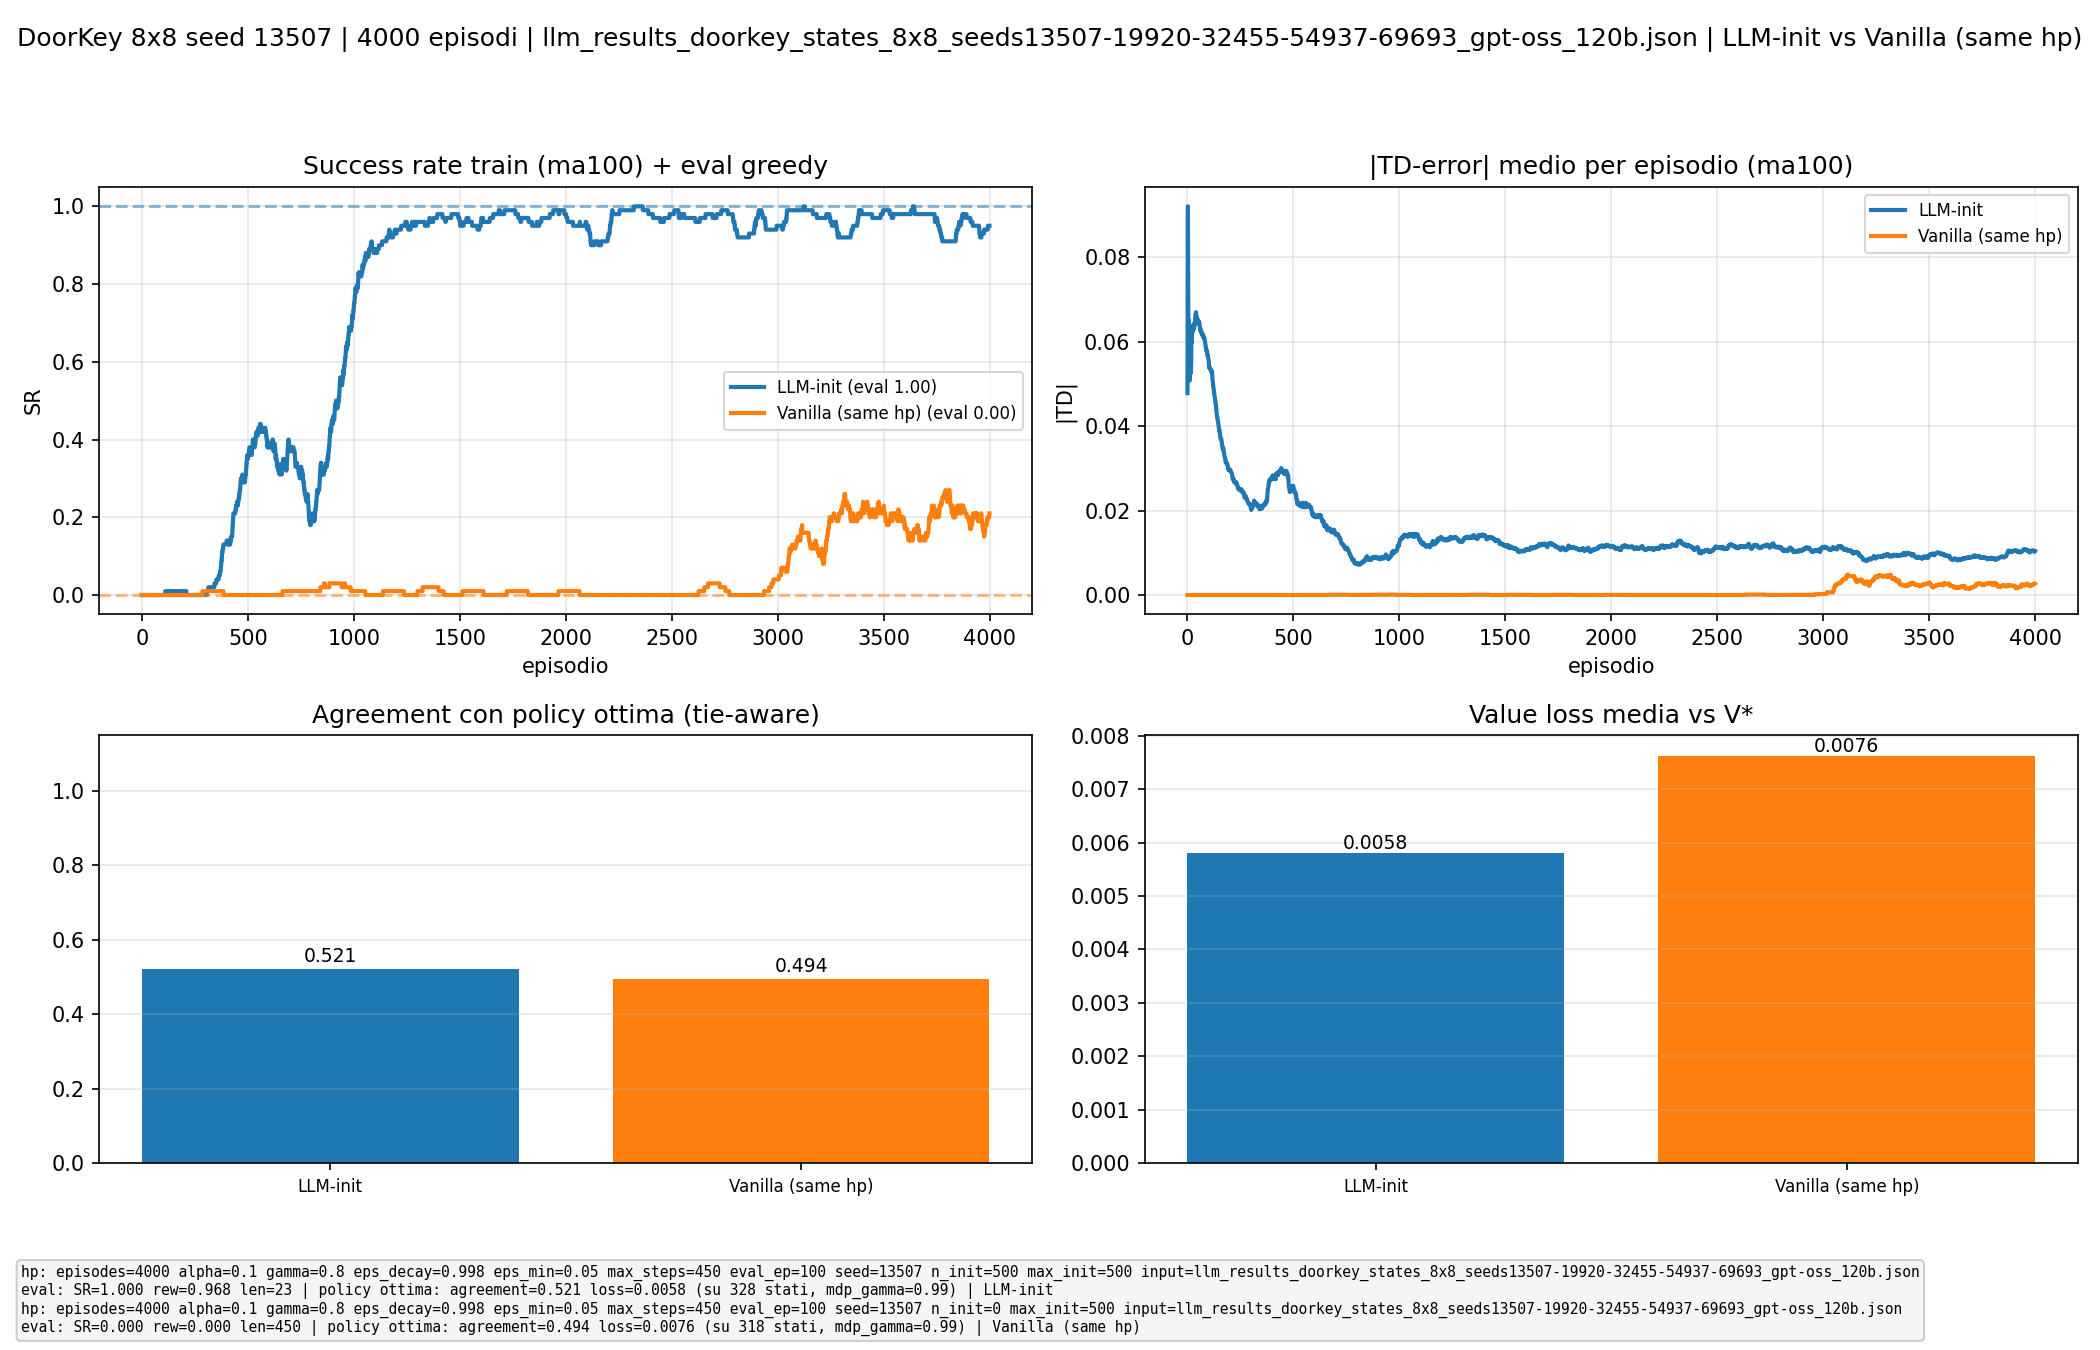
\includegraphics[width=\textwidth]{../src/output/agents/qtable_llminit_multiseed_train13507-19920-32455-54937-69693_evalin13507_evalnew6499_vs_samehp.png}
\caption{Multi-seed, confronto a pari iperparametri: il controllo resta a zero e sul seed nuovo non si osserva trasferimento.}
\label{fig:multisamehp}
\end{figure}

\begin{figure}[htbp]
\centering
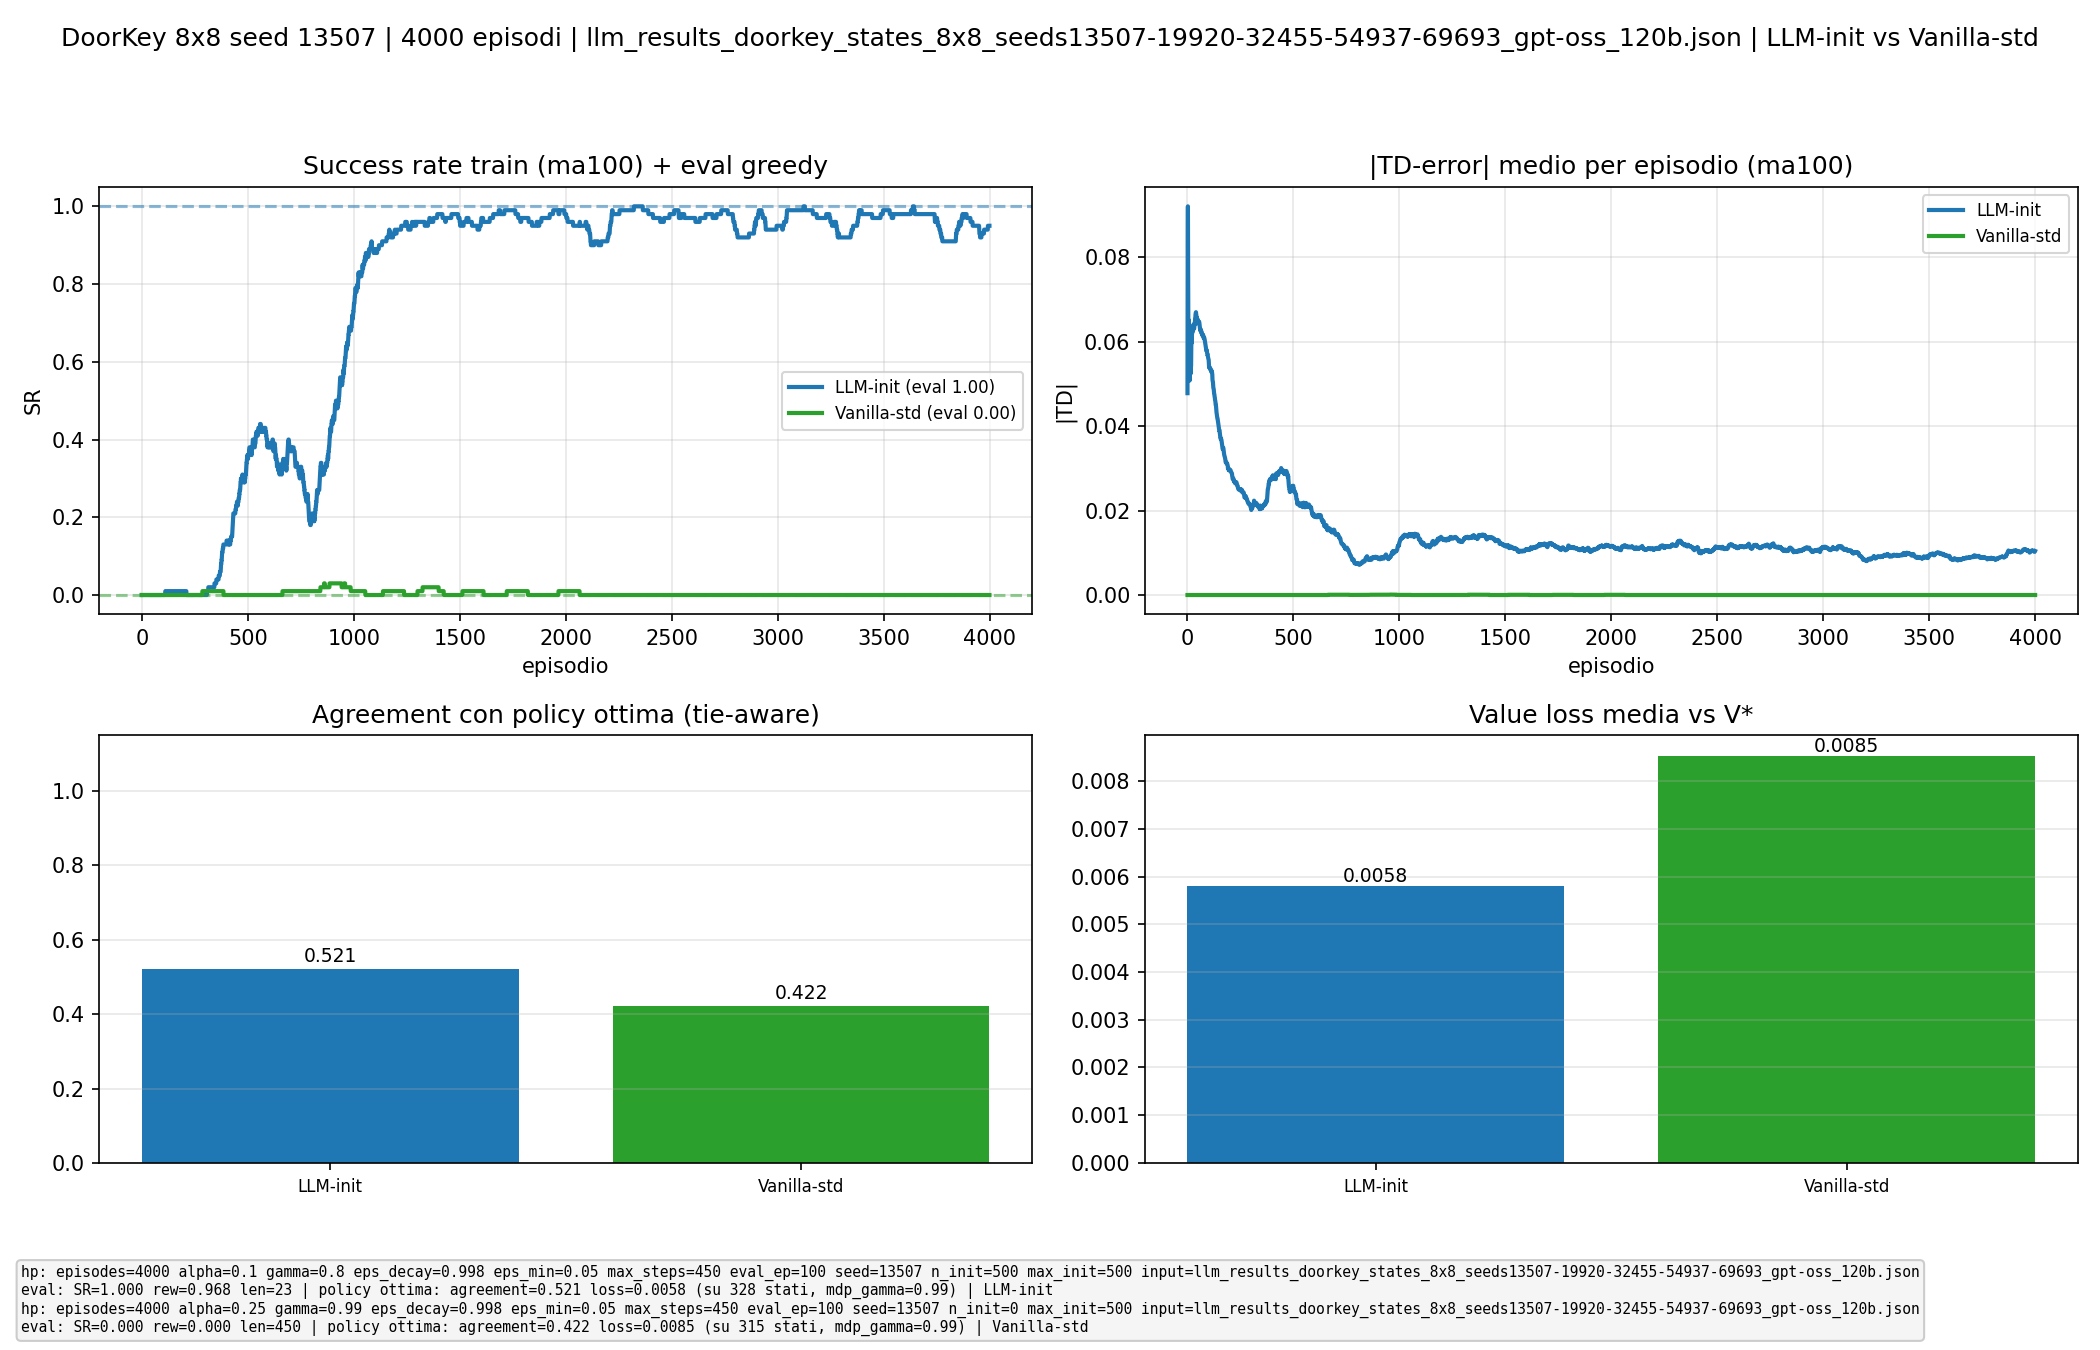
\includegraphics[width=\textwidth]{../src/output/agents/qtable_llminit_multiseed_train13507-19920-32455-54937-69693_evalin13507_evalnew6499_vs_std.png}
\caption{Multi-seed, confronto con il controllo a iperparametri standard: il controllo resta a zero su entrambi i seed.}
\label{fig:multivstd}
\end{figure}

Esperimenti preliminari con $\alpha=0.2$, $\gamma=0.95$, 1500 episodi: con 720 coppie il primo successo arriva all'episodio 14 con 13 passi finali (l'ottimo); con 50 coppie arriva al 40; senza inizializzazione arriva al 127 con valutazione 0.00. Una maggiore quantit\`a iniziale anticipa la curva di apprendimento, a parit\`a di punto di arrivo.

Le stime sono prodotte con $\gamma=0.99$ mentre l'agente opera a 0.9 o 0.95: l'inizializzazione risulta approssimata sotto due aspetti e mantiene comunque efficacia.

\section{Iperparametri}\label{sec:iperparametri}
La configurazione principale impiega $\alpha=0.07$, $\gamma=0.9$, decadimento di $\epsilon$ 0.99 con minimo 0.05 e limite di 450 passi, per i motivi seguenti:
\begin{itemize}
\item $\gamma=0.9$ invece di 0.99. Con 0.99 due stati vicini differiscono del fattore 0.99, con ridotta discriminabilit\`a per la politica greedy. Con 0.9 il gradiente indotto dai valori iniziali risulta pi\`u marcato. Nell'analisi di sensibilit\`a: con $\gamma=0.99$ il regime si raggiunge solo all'episodio 770 con 16 passi, con $\gamma=0.9$ e $\alpha=0.5$ all'episodio 286 con 13 passi.
\item $\alpha$ ridotto. La tabella parte prossima ai valori di riferimento, pertanto incrementi contenuti consentono un affinamento senza alterare l'inizializzazione. Con $\alpha=0.9$ l'avvio \`e rapido ma il consolidamento \`e successivo (episodio 350 contro 289).
\item decadimento di $\epsilon$ pari a 0.99 con minimo 0.05. L'esplorazione risulta prolungata ma limitata. Il limite di 450 passi consente le deviazioni iniziali: l'ottimo \`e 13 passi, mentre nelle fasi iniziali risultano necessari ordini di grandezza superiori.
\end{itemize}
La combinazione con consolidamento pi\`u rapido \`e $\alpha=0.5$, $\gamma=0.9$: primo successo all'episodio 5, regime all'episodio 286, 13 passi finali.

\section{Limiti}\label{sec:limiti}
Primo: mappe non osservate. L'esperimento multi-seed della Sezione~\ref{sec:init} ottiene tasso 1.00 sui seed di addestramento ma 0.00 sul seed nuovo: cinque seed non bastano, per generalizzare ne servono molti di pi\`u. La coordinata relativa riduce lo spazio ma non rappresenta muri e strozzature, che variano con il seed. Tale punto costituisce il limite principale. L'ampliamento di seed e stati risulta utile solo a condizione che la rappresentazione sia adeguata. Il costo resta pari a una interrogazione al modello per stato.

Secondo: caso degenere dell'esecuzione preliminare (Sezione~\ref{sec:stati}). Su due seed su sei i checkpoint coincidono temporalmente e non descrivono una traiettoria di apprendimento.

Terzo: scala e costo. La quota campionata su un grafo di 480 nodi risulta sufficiente sulla 8x8. Su mappe maggiori la frazione utile decresce e le interrogazioni al modello restano la fase di maggiore durata.

\section{Sviluppi futuri e conclusioni}\label{sec:conclusioni}
Sul 1337: errore 0.0122 con 94.1\% di azioni ottime e valutazione da 0.00 a 1.00 a pari iperparametri con 20 coppie. Sui cinque seed: errore 0.0153 con 91.9\% di azioni ottime e tasso interno a 1.00 con 23 passi. Sul seed nuovo: 0.00. Il limite, descritto nella Sezione~\ref{sec:limiti}, consiste nell'assenza di trasferimento.

Restano tre sviluppi da verificare:
\begin{enumerate}
\item \textbf{Addestramento completo su molti pi\`u seed.} Cinque seed danno tasso 1.00 sui layout visti e 0.00 sul nuovo: per generalizzare serve un addestramento completo che copra molti pi\`u layout, affinch\'e la politica risultante tenga su mappe non osservate.
\item \textbf{Modello affinato per risposte rapide.} Un modello fine-tuned sullo specifico caso d'uso, in grado di restituire i valori della funzione in modo molto veloce, ridurrebbe il costo unitario per stato che oggi rende impraticabile l'interrogazione su larga scala.
\item \textbf{Stime generate durante l'addestramento.} Anzich\'e stimare i valori una sola volta prima di iniziare, il modello verrebbe interrogato sui nuovi stati incontrati, guidando l'esplorazione in corso d'opera.
\end{enumerate}
Per vincoli di costo gli esperimenti presentati sono in singola esecuzione e i risultati sono da intendersi come prova di fattibilit\`a.

\appendix
\section{Appendice: ambiente FrozenLake}\label{sec:frozenlake}
La medesima ipotesi \`e applicata all'ambiente \path{FrozenLake-v1} 8x8 in modalit\`a stocastica, senza fasi. La procedura \`e predisposta nei moduli dedicati (grafo, interrogazione sui bottleneck, valutazione, agente); i dati non sono versionati e se ne descrive esclusivamente l'architettura.

Il modello da 120 miliardi di parametri su 18 bottleneck riporta errore 0.1228, scelte giuste al 55.6\% contro 25\% del livello casuale, rimpianto 0.0060. Il modello da 26 miliardi riporta errore 0.3383 e scelte giuste al 77.8\%, con valori fuori scala. Pochi stati e misure deboli: lavoro in corso, non risultato acquisito. La causa probabile risiede nella natura stocastica di $Q^*$ con scivolamento, a fronte di una singola stima per tre esiti possibili.

\begin{thebibliography}{9}
\bibitem{sutton2018} Sutton, R.~S., Barto, A.~G. \textit{Reinforcement Learning: An Introduction}, 2nd ed., MIT Press, 2018.
\bibitem{minigrid2023} Chevalier-Boisvert, M. et al. MiniGrid and MiniWorld. \textit{NeurIPS} 36, 2023.
\end{thebibliography}

\end{document}
